\chapter{Design of DevOps Toolchains}
In this chapter, we will introduce the design and implementation of DevOps toolchains.
Note that for the experiment that is answering RQs in Chapter 5, we implement two different continuous delivery pipelines design with two sets of tools respectively, one with tradition non-integrated tool while another one with the serverless integrated DevOps tools from AWS. In conclusion, we introduce the design of both toolchains(integrated and non-integrated) and explain how we come to this implementation in this chapter.
We will also compare these two types of toolchains within the scope of functionality and ease of implementation.
\par
In Section 4.1, we present the case software project developed by us that will be built, tested, and deployed by our DevOps toolchain in the experiment. In section 4.2, we introduce the design and implementation of our non-integrated DevOps toolchain. Section 4.3 is related to the integrated toolchain, and section 4.4 is a comparison between Integrated and non-integrated toolchain. Lastly, in section 4.5, we talk about the challenges we met during the implementation.
\section{Case Project}
We first develop the case project. The case project is an example software project which will be used to test our implementation and run the experiments in which we simulate the DevOps development process of the case project on our DevOps toolchain. Although the type of our case project has no effect on our DevOps toolchain on the architecture level, the build dependencies and the software configuration inside our toolchain could be affected by it. Thus we must have an introduction to the case project.
\subsection{Programming Language and Framework Considerations}
Java is one of the most common languages used in commercial software development. According to the TIOBE index of programming language \cite{indexTIO42:online}, Java is the most popular or the second most popular programming language in the world since the mid-1990s. Besides commercial software development inside companies, Java programming language is widely used in open-source software development. The report \cite{TheState3:online} from GitHub shows that Java ranked third most popular programming language in 2019, and it ranks second before 2018. Furthermore, Java has good versatility, which means it almost every kind of applications. For instance, web applications, desktop applications, besides, Java is the main development language for Android applications.
\par
To the DevOps point of view, the Java programming language has a complete ecosystem. The complete ecosystem means there are tools for every phase of Java application development. These tools include: build, code analysis, testing frameworks, artifact management, build automation \& dependency management et. These tools could be easily integrated and act as part of the DevOps toolchain.
\par
Hence, due to the popularity, versatility and complete ecosystem of Java programming language, we select Java as the language of the case project.
\par
One of the major application of Java in web development. Currently, 7 out of 10 \cite{Programm17:online} most popular website is using Java as a web development language (server-side). In the field of web development, Spring framework is the most popular framework for Java, and it is being used in many major internet companies including Google, Microsoft and Amazon \cite{SpringWh14:online}.
\par
So, we choose Spring the framework to build our application. To develop our Spring application, we use Spring Boot\footnote{https://spring.io/projects/spring-boot}. Spring Boot is a project under Spring, which, according to its documentation, is to allow the developer to create Spring application with the minimal effort \cite{SpringBo84:online}, by simplifying the configuration of Spring framework.
\subsection{Project Description}
\begin{figure}[!h]
\begin{verbatim}
Method: GET
Endpoint: /packages
Success Response:
Code: 200
Content:
[
{
name : (Package name)
description : (Package description)
dependencies : (Dependencies)
}
]
Error Response:
Code: 500
Content: { msg: Server Error! }
\end{verbatim}
\label{fig:rest}
\caption{RESTful API Interface of Case Project}
\end{figure}
The case project is a simple REST API (Figure \ref{fig:rest}) which returns the info of all installed software packages in the host machine in JSON format when the frontend sends an HTTP GET request to the backend.
\section{Design of Non-integrated DevOps Toolchain}
In section, we present our design of non-integrated DevOps toolchain. Part of the components is still based on the virtual machine those we cannot call it a serverless toolchain as in the integrated toolchain. Each section is the introduction to the design of each component. We also present the consideration when a select tool for this part of the toolchain in each section. Besides, in each section, we introduce how could serverless computing be used by this component in general and the benefits to the specific tool we select.
\subsection{Architecture}
The toolchain implementation is based on the DevOps elements we presented in Chapter 2, and the DevOps practises from Eficode. Figure \ref{fig:archjenkins} shows the architecture of our DevOps toolchain. In here we are only presenting architecture on a more general level. The detailed architecture of each component will be introduced in the following sections, both text and graph.
\par
When the developer pushes a new commit to the repository in GitHub \footnote{https://github.com/}, Github will send HTTP POST request that contains the necessary information to the Jenkins master node. Jenkins master, which triggered by the HTTP request, will create a new job for this project according to the information that the HTTP request contains. The job will first pull the latest code from the git repository, then runs the docker containers with required build environment and build the project. In the end, a docker image for running the project will be created and be pushed to the container registry of AWS. Depends on the git branch that the developer committed to, the project will be deployed to a different development environment.
\begin{figure}[h]
     \centering
     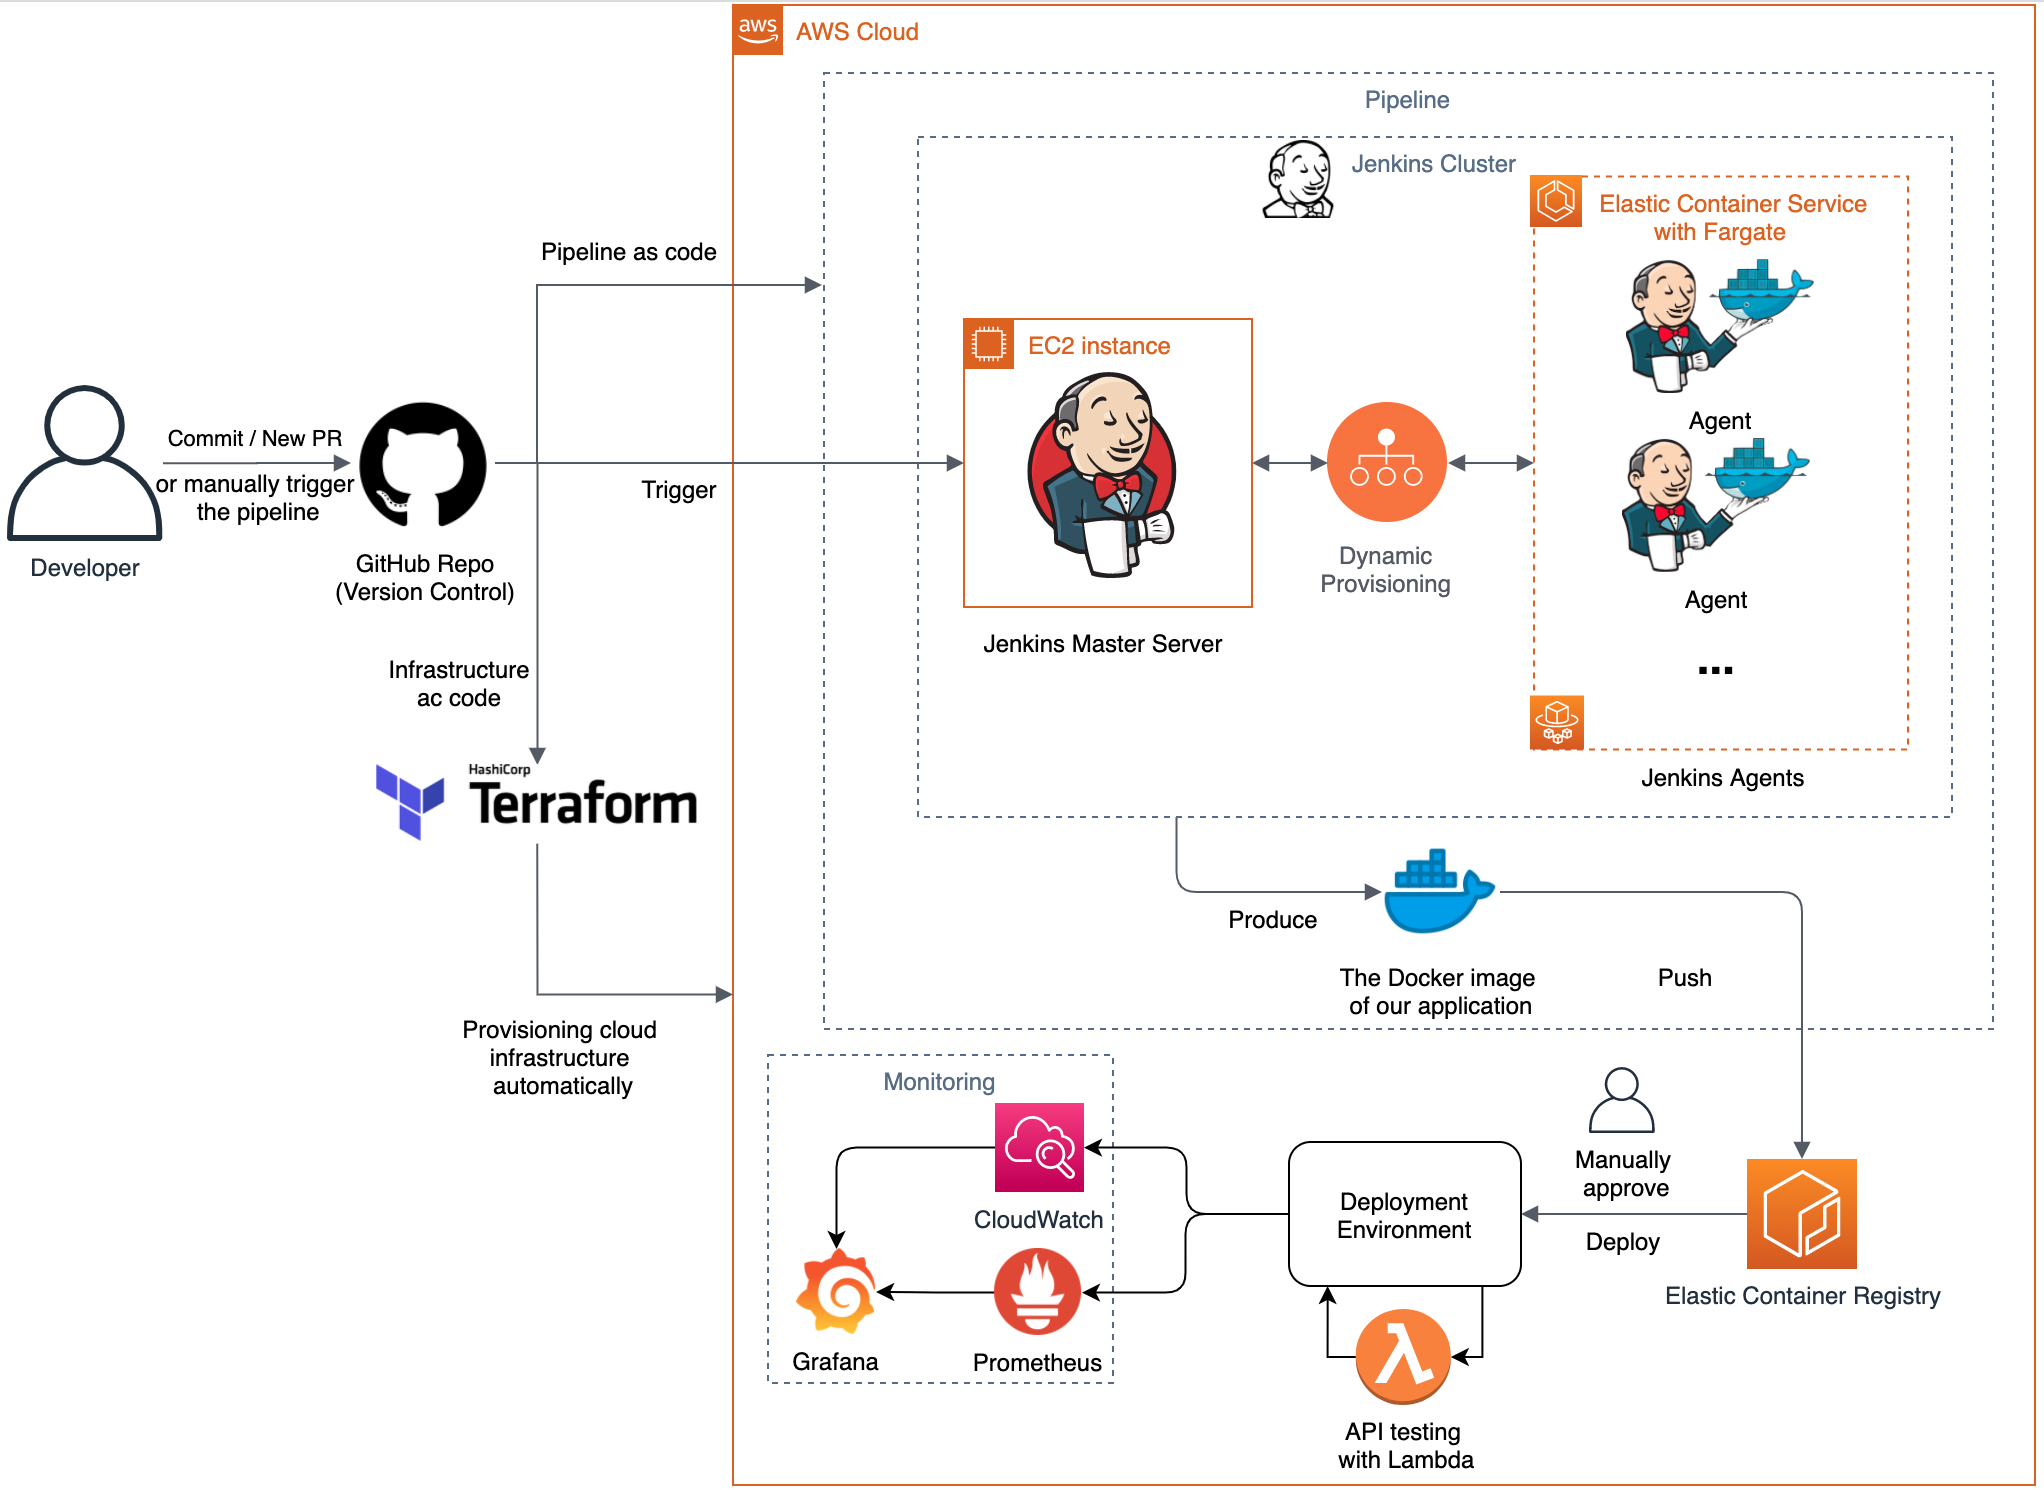
\includegraphics[width=0.99\textwidth]{pics/arch-med-jenkins.png}
     \caption{Architecture diagram of the non-integrated DevOps toolchain}
     \label{fig:archjenkins}
     \end{figure}
\par
Figure \ref{fig:archjenkins} shows the architecture of our DevOps toolchain. We can see except version control, and the whole environment is running in Amazon Web Services. Due to the limitation of space, the internal architecture of certain components is not shown in the graph. Instead, we show them in the following sections.
\subsection{Introduction to Tools Used in the Implementation}
One of the essential steps to build the non-integrated toolchain is to select the proper tool for each component.
In this section, we describe our consideration when we select tools.
\paragraph[]{Continuous Delivery Pipeline}
The most popular server-based tools for build continuous delivery pipeline are Jenkins\footnote{https://www.jenkins.io/}, Drone\footnote{https://drone.io/}, GoCD\footnote{https://www.gocd.org/} and Circle CI\footnote{https://circleci.com/}. Table \ref{tab:ci-tools} shows a comparison between these tools. As we can see from the table, Jenkins is the most popular option for CI/CD. Jenkins has wide application in the commercial use case, and the high popularity in the open-source community as well. Although compared with the other three newer tools, Jenkins is more focuses on the "Build" step within the continuous delivery pipeline since it was originally a build automation server. But, the open-source nature of Jenkins gives it a much wider selection of the plugin, which means Jenkins can be used for almost all steps in a continuous delivery pipeline.
\begin{table}[h]
\begin{tabular}{|l|l|l|l|l|}
\hline
& Jenkins & Drone & Circle CI & GoCD \\ \hline
Open Source & Yes & Yes & No & Yes \\ \hline
GitHub stars & 15.7k & 21.2k & - & 5.7k \\ \hline
Github contributors & 614 & 258 & - & 116 \\ \hline
Plugin extensions &
Over 1500 \tablefootnote{https://plugins.jenkins.io/} &
93 \tablefootnote{According to GitHub search result} &
110 \tablefootnote{https://circleci.com/integrations/} &
88 \tablefootnote{https://www.gocd.org/plugins/} \\ \hline
\begin{tabular}[c]{@{}l@{}}Price of self-hosted \\ solution\end{tabular} &
Free &
Free &
\$35 user/month &
Free \\ \hline
\begin{tabular}[c]{@{}l@{}}Number of companies\\use it in the tech stack\tablefootnote{based on data from StackShare}\end{tabular} &
2634 &
82 &
1368 &
42 \\ \hline
\end{tabular}
\caption{Comparison of continuous delivery tools}
\label{tab:ci-tools}
\end{table}
\par
Created by Kohsuke Kawaguchi in 2001, Jenkins is an open-source continuous integrating tool write with Java. It is suitable for a team of all sizes and varies of languages and technologies \cite{smart2011jenkins}. Furthermore, Jenkins also attracts software teams with its easy-to-use and high extendibility \cite{smart2011jenkins} with a thousand of the plugin. More plugin keeps coming since Jenkins has an active open-source community. These plugins help Jenkins keep up with the fast-developing DevOps practices, and help Jenkins integrate with the newly emerging tools and cloud services. The extendibility makes Jenkins still the most popular tool for DevOps toolchain even it is an aged software created when the term "DevOps" just appeared.
\par
Our continuous delivery pipeline is developed with Pipeline plugin\footnote{https://www.jenkins.io/doc/book/pipeline/} in Jenkins.
Pipeline plugin allows us to define a continuous delivery pipeline as code in Jenkinsfile.
In the pipeline, a conceptually distinct subset of tasks within the continuous delivery pipeline \cite{Pipeline85:online} is defined as a "stage"\footnote{For example, "Build", Test", "Deploy" step in a continuous delivery pipeline.} and each task within a step is called "step". Each pipeline is binding with a "project". An execution runtime of a project/pipeline is called "build", and the machine (virtual machine, container, e.t.) for running the build is called "agent".
\paragraph[]{Build \& Test Automation Tool}
For the build stage within Jenkins pipeline, we use Gradle\footnote{https://gradle.org/} as the build tool.
Gradle is a powerful build tool initially designed for JVM based language, but now it also supports other programming languages, for example, C++ and Python. Like Jenkins, Gradle also has a dynamic ecosystem with thousands of plugin. This enables the possibility to use different kinds of tools such as unit testing and code analysis within a single pipeline of Gradle. Gradle also makes the dependency management easy, and dependencies could be easily added to the project by editing the Gradle configure file of the project. Furthermore, Gradle supports configuration as code. This allows developers to define all the build configurations of a software project in a single file.
\par
For unit testing within the build stage, we are using JUnit \footnote{https://junit.org/junit5/} as the tool for testing. For code analysis, we use SonarQube\footnote{https://www.sonarqube.org/}. Both are one of the most common used tools in their specialized field in the Java ecosystem. Moreover, both tools have official Gradle plugin, which allows us easily use them with Gradle.
\paragraph[]{Deployment and Jenkins Agents}
We will widely use Docker \footnote{https://www.docker.com/} in our pipeline.
Docker is an open-source software which could pack, deliver and run the software as a container. A container is a separate unit that includes the application and all its dependencies which allow application runs in the same way regardless of the host environment \cite{WhatisaC60:online}. A container is the running instance of a Docker image that defined by Dockerfile.
\par
\label{docker}
There will be two main use cases of Docker in our toolchain. Firstly, we run the build stage within the container.
Nowadays, Docker\footnote{https://www.docker.com/} is being widely used as build agents in continuous integration and continuous delivery (CI/CD) pipelines.
This means the pipeline will execute specific steps inside ephemeral Docker containers \cite{Overview44:online}. It is easier to manage build dependencies in the Docker container. Besides, the container-based agent requires less effort to maintain.
\par
In our case, to build the case application, the host machine needs to have JVM installed. However, we want to make our pipeline not only suitable for Java application but also easily be used to build an application in other programming languages. Docker solves this problem by provides excellent isolation from the host machine. Thus, we can configure the built environment (operating system version, dependencies) runs within a Docker container without actually install anything on the host machine by merely editing the Dockerfile.
\par
We also use Docker to Dockerize our application which creates a Docker image of our application.
Docker allows us to specify all system dependencies in a single file (Dockerfile), so there is no need to have any Java environment pre-installed in the deployment environment which runs our application. This is because all environment is already being packed in our Docker image. By doing this, firstly, we reduce the operational effort. Secondly, we improve compatibility since Docker makes sure that the docker image could run in the same behaviour no matter what host machine it runs on. Also, all major cloud computing providers support Docker. We could easily run the container from our Docker image on their VM, and they are serverless computing services. This means our Dockerized application could easily be cloud-native and be deployed across a multi-cloud environment.
\paragraph[]{Monitoring}
We using CloudWatch for monitoring the status of the cloud infrastructure. CloudWatch is an tools provided by AWS, which we already introduced in Chapter 3. However, It's not possible for CloudWatch to give us insight about the status of Java SpringBoot application. More generally, the metrics within the application framework. In Spring Boot, these metrics are HTTP statistics, CPU load and JVM statistics. Prometheus \footnote{https://prometheus.io/}, together with Grafana could fill this gap.
\par
Prometheus is an open source monitoring and alerting solution initially built by SoundCloud in 2012 \cite{Overview30:online}. Prometheus is used for reading numeric metrics that are recorded in time series. In Spring Boot, there are some plugins ,for example, Micrometer \footnote{https://micrometer.io/} exist which could export all the Spring Boot specific metrics to Prometheus in time series. Thus Prometheus has perfect fit with our case project. In addition to collecting metrics, we could also set alarm within Prometheus, which could alert user when some metrics are not in normal range. We can also query the metrics from the past. Although Prometheus supports simple graph which show the metrics' change with time, it is not user friendly enough. Thus, we introduce Grafana to better visualizes the data collected by Prometheus.
\par
Grafana is a observation platform which it's core feature is in the visualization. Users could define dashboards according to their needs with JSON files. Another main feature if Grafana is that it could gather data from different platform into one dashboard. In our case, with Grafana, we can display the metrics from Prometheus and CloudWatch in a single page. This could gives us great overview to both Spring Boot application and cloud infrastructure as the same time.
\subsection{Infrastructure as Code (IasC)}
Configuration Management is one of the component of DevOps toolchain that we mentioned in Chapter 2. Infrastructure as code the common practices to implement configuration Management in the cloud-based environment.
\begin{figure}[h]
\centering
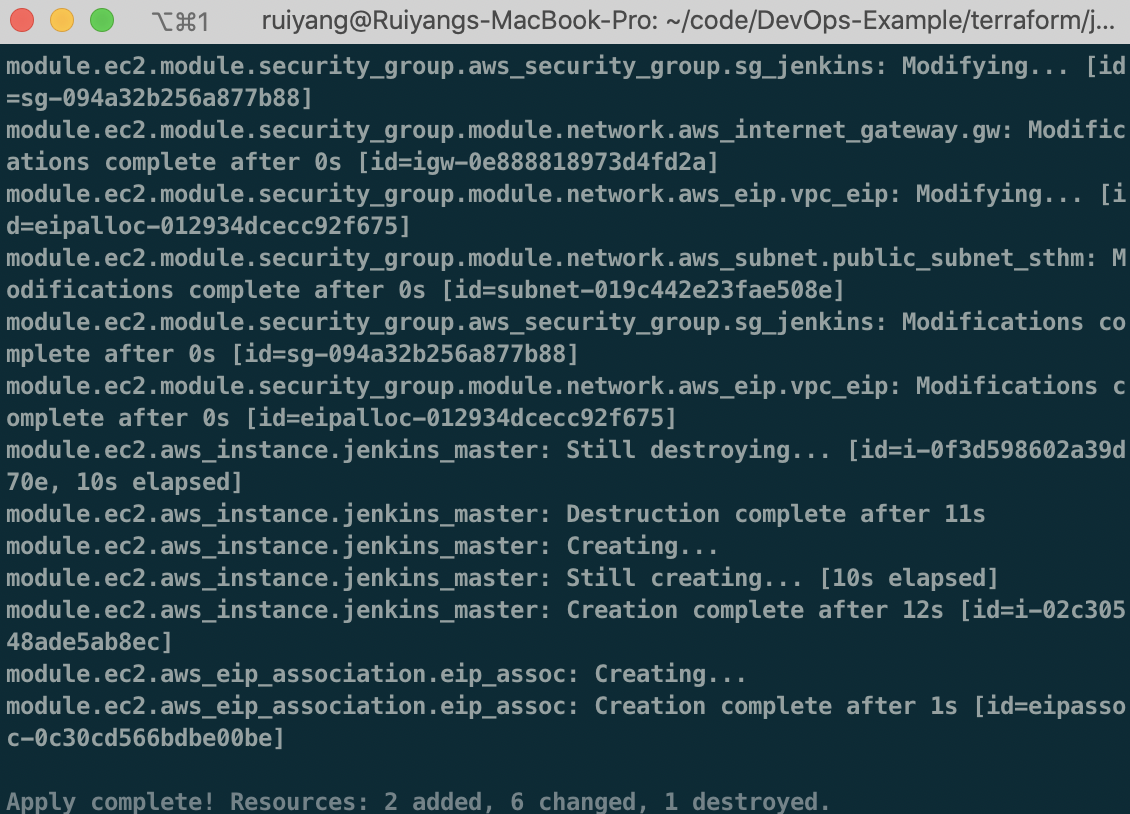
\includegraphics[width=0.99\textwidth]{pics/terraform.png}
\caption{Creating a cloud environment with Terraform CLI}
\label{fig:terraform}
\end{figure}
\par
Terraform \footnote{https://www.terraform.io/} is one of the most popular tools to manage cloud Infrastructure with IasC practice. It has the thorough support of AWS. In our implementation, we define our could infrastructure and all AWS resources including EC2 virtual machine, ECS cluster, security groups and network Infrastructures in a series of configuration files. Then we create the cloud environment by simply using CLI interfaces. Figure \ref{fig:terraform} shows the creation of the cloud environment with Terraform.
\subsection{Version Control}
Version Control System (VCS) is the process that record the changes in files set over time \cite{GitAbout93:online}, and versioning the history of these files. VSC is suitable for track the development progress and manages the goal within a software development team \cite{loeliger2012version}. Among all software for version control, Git is the most popular one nowadays. The survey \cite{CompareR31:online} from Synopsys shows that in 2019, 71\% of the project today is using Git as it is versioning system while SVN that ranks in second only be used in 25\% of the projects. We use Git as the version control system since it is used by most of the software development teams nowadays. We use GitHub for hosting the case project. Github is the biggest preform in the world that hosting a version-controlled software project for free using Git. It provides interfaces with different DevOps related tools which makes it easy to be integrated into all kinds of DevOps toolchains.
\begin{figure}[h]
\centering
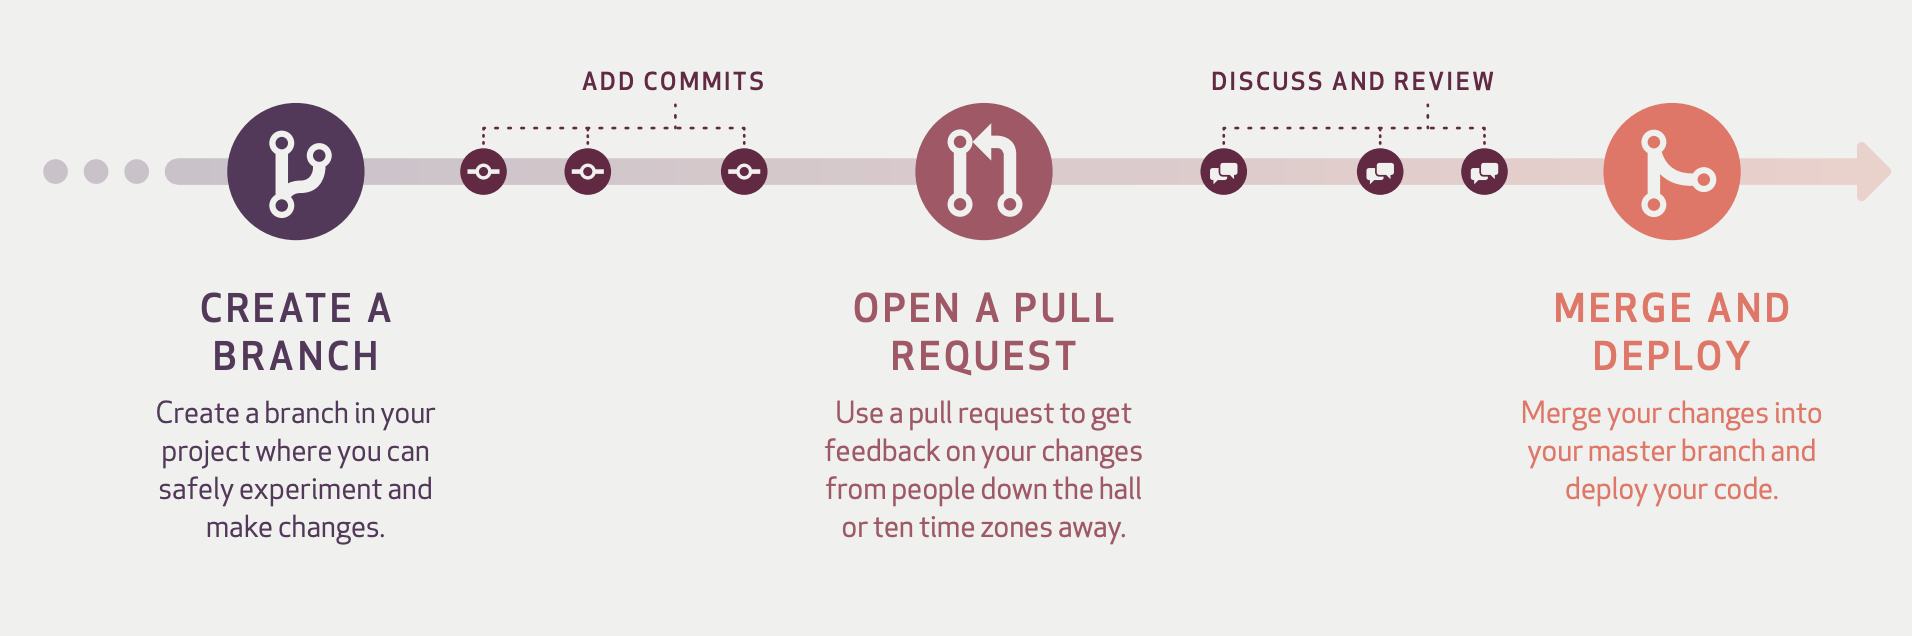
\includegraphics[width=0.99\textwidth]{pics/git.png}
\caption{GitHub Workflow \cite{guides2013understanding}}
\label{fig:git}
\end{figure}
\par
The Git flow \cite{driessen2010successful} proposed in 2010 is a successful workflow for working with Git. Git flow has already widely used and has been approved by the software industries. However, to better cope with the frequent release nature of DevOps, the Github workflow -- a simplified version of Git flow is proposed by GitHub.
Therefore, GitHub workflow \cite{chacongithub} is being chosen as our workflow in the version control. The simplified version of this workflow is shown as in Figure \ref{fig:git}
\par
Several general principles followed by us when adapting GitHub flow, we refer to principals in \cite{chacongithub} to design our workflow.
\begin{itemize}
\item Master branch is always deployable. This means when deploying the continuous delivery pipelines in our toolchain, only the master branch can be deployed. Moreover, there should not have any code which is not good to be deployed in the master branch.
\item When working on the new feature, make a new branch for this feature. The name of this branch should be descriptive, which reflect the content of this feature. Commit the new code related to this feature to the feature branch. And push from this feature branch to the branch with the same name on the remote server (github.com) when necessary.
\item Open a pull request\footnote{https://help.github.com/en/GitHub/collaborating-with-issues-and-pull-requests/about-pull-requests} when the feature is ready to merge, or when developer feel that he/she need help or comments from other team means on this feature. Others also do the code review in the pull request.
\item When the code is reviewed and is good to be merged, the developer should merge the code to the master.
\item After the code of this feature is in the master, the code will and should be immediately deployed. There should not be any rollback in the master branch. If there are any issues within the newly merged code, a new commit or a new branch should be made to fix the issue rather than rollback on the master.
\end{itemize}
\par
Note that in our Git workflow, there are several time points that we need to run the continuous delivery pipeline within the toolchain. The continuous delivery pipeline will also vary with the time point within the version control workflow. We will introduce this in detail on \ref{our-ci}.
\subsection{Continuous Delivery Pipeline}
\label{our-ci}
\begin{figure}[h]
 \centering
 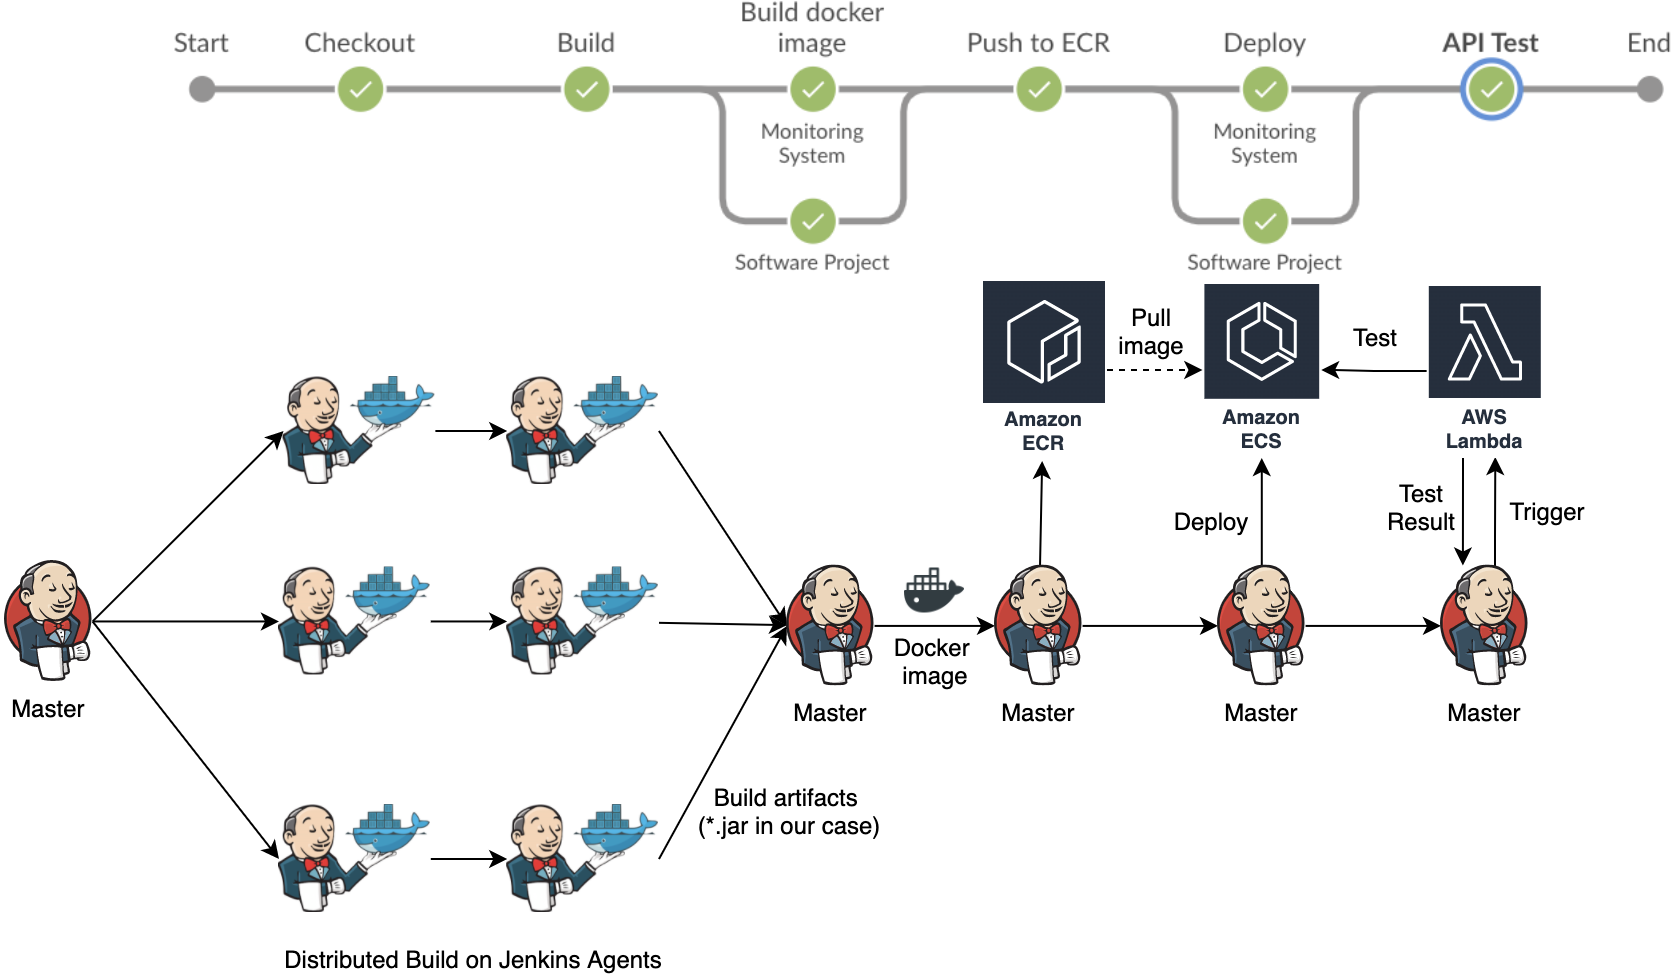
\includegraphics[width=0.95\textwidth]{pics/overview.png}
 \caption{The Stages and Distributed Build in Our Pipeline}
 \label{fig:overview}
\end{figure}
Figure \ref{fig:overview} shows the six Jenkins stages in our pipeline. The bottom part of this Figure shows the task distribution between the master node and agent nodes. The master node is an EC2 virtual machine while agents run on Fargate instances within an ECS cluster. In section 2.3.1 we mentioned that the development of the monitoring system should be in parallel with the main software project, thus in our pipeline, the build and deploy of monitoring system is in parallel with the case project.
\par
As we can see from the Figure, when the master node starts a job, it will create a Docker container in AWS Fargate as the agent. The agent will pull codes from VCS, build the code, and then send the build artifacts back to the master node. After this, the container will be terminated. The master node will continue the rest steps.
\paragraph[]{Build Agents}
Build agent is an independent computation unit (VM or Docker container) that could exchange data with the Jenkins master node and run a certain part of the pipeline. To implement a Jenkins build cluster, we need first to implement build agents.
We discussed why we use Docker-based agent in our Jenkins build a cluster on \ref{docker} and we decide to it in our implementation. The first step of our implementation is to develop our own Docker image \footnote{The Docker image we developed could be found at https://hub.docker.com/r/dry1995/jnlp} of the Jenkins agent. We use the "jenkins/jnlp-slave"\footnote{https://hub.docker.com/r/jenkins/jnlp-slave/} as the base image, this allows our Jenkins agent to establish an inbound connection to the Jenkins master with TCP. The next step is to set up the built environment within the agent. We add shell script for auto-install all build dependencies of our case project when we build this Docker image. In the last step, we build the Docker image for build agent and push it to DockerHub. 
\par
We also discussed how Fargate allows us to run container serverlessly. To make use of Serverless offering of AWS, we let Docker-based Jenkins agents run on AWS Fargate to cut the operational effort and automate the scaling of Jenkins cluster. To implement this, we use Jenkins plugin "Amazon Elastic Container Service (ECS) / Fargate", which is the only Jenkins plugin allow us to host Jenkins agent in Fargate.  
\paragraph[]{Considerations in Designing the Workflow of Distributed Pipeline}
The considerations behind to our design are that the first two steps take most of the time in our pipeline and according to Figure \ref{fig:pipeline} runs more frequently than other steps \footnote{The reason will be discussed in next section "Workflow in Production"}. The running time will be further extended when building a larger project. These two stages will be the bottleneck of the pipeline if we have it on the master mode. So we need to offload these steps to Jenkins agents for better performance.
\par
The second reason is: as we mentioned in our introduction of Docker at \ref{docker}, the built environment inside the Jenkins agent that runs in Docker container is easier to be changed. When the team want to build the same code for different OS (Which happens in C/C++ development) or want to have a different build environment for different projects, they eliminate tasks such as configuration and installation different environment thanks to Docker. Instead, they can just modify the Dockerfile that defines the Docker image of the Jenkins agents. However, we cannot put the stage that builds a Docker image in Jenkins agents. This is because AWS Fargate does not allow building agent runs in a free container which means we cannot use Docker within the Jenkins agent's container that runs in Fargate. This is one significant limitation of Fargate, so we have to move the step back to the master node. Fortunately, in our case project, the Docker build only takes a short time (<1s on average). Therefore this will not slow down the whole pipeline.
\par
We also notice that the Deploy stage also takes a long time. Still, we do not have it in the distributed build because: first, it is on the end of a pipeline so it will not block the further steps, second, the pipeline runs the stage less frequently than first two stages as shown in Figure \ref{fig:pipeline}. Thus there will be less possibility that there are many jobs runs at "Deploy" stage in parallel.
\begin{figure}[h]
 \centering
 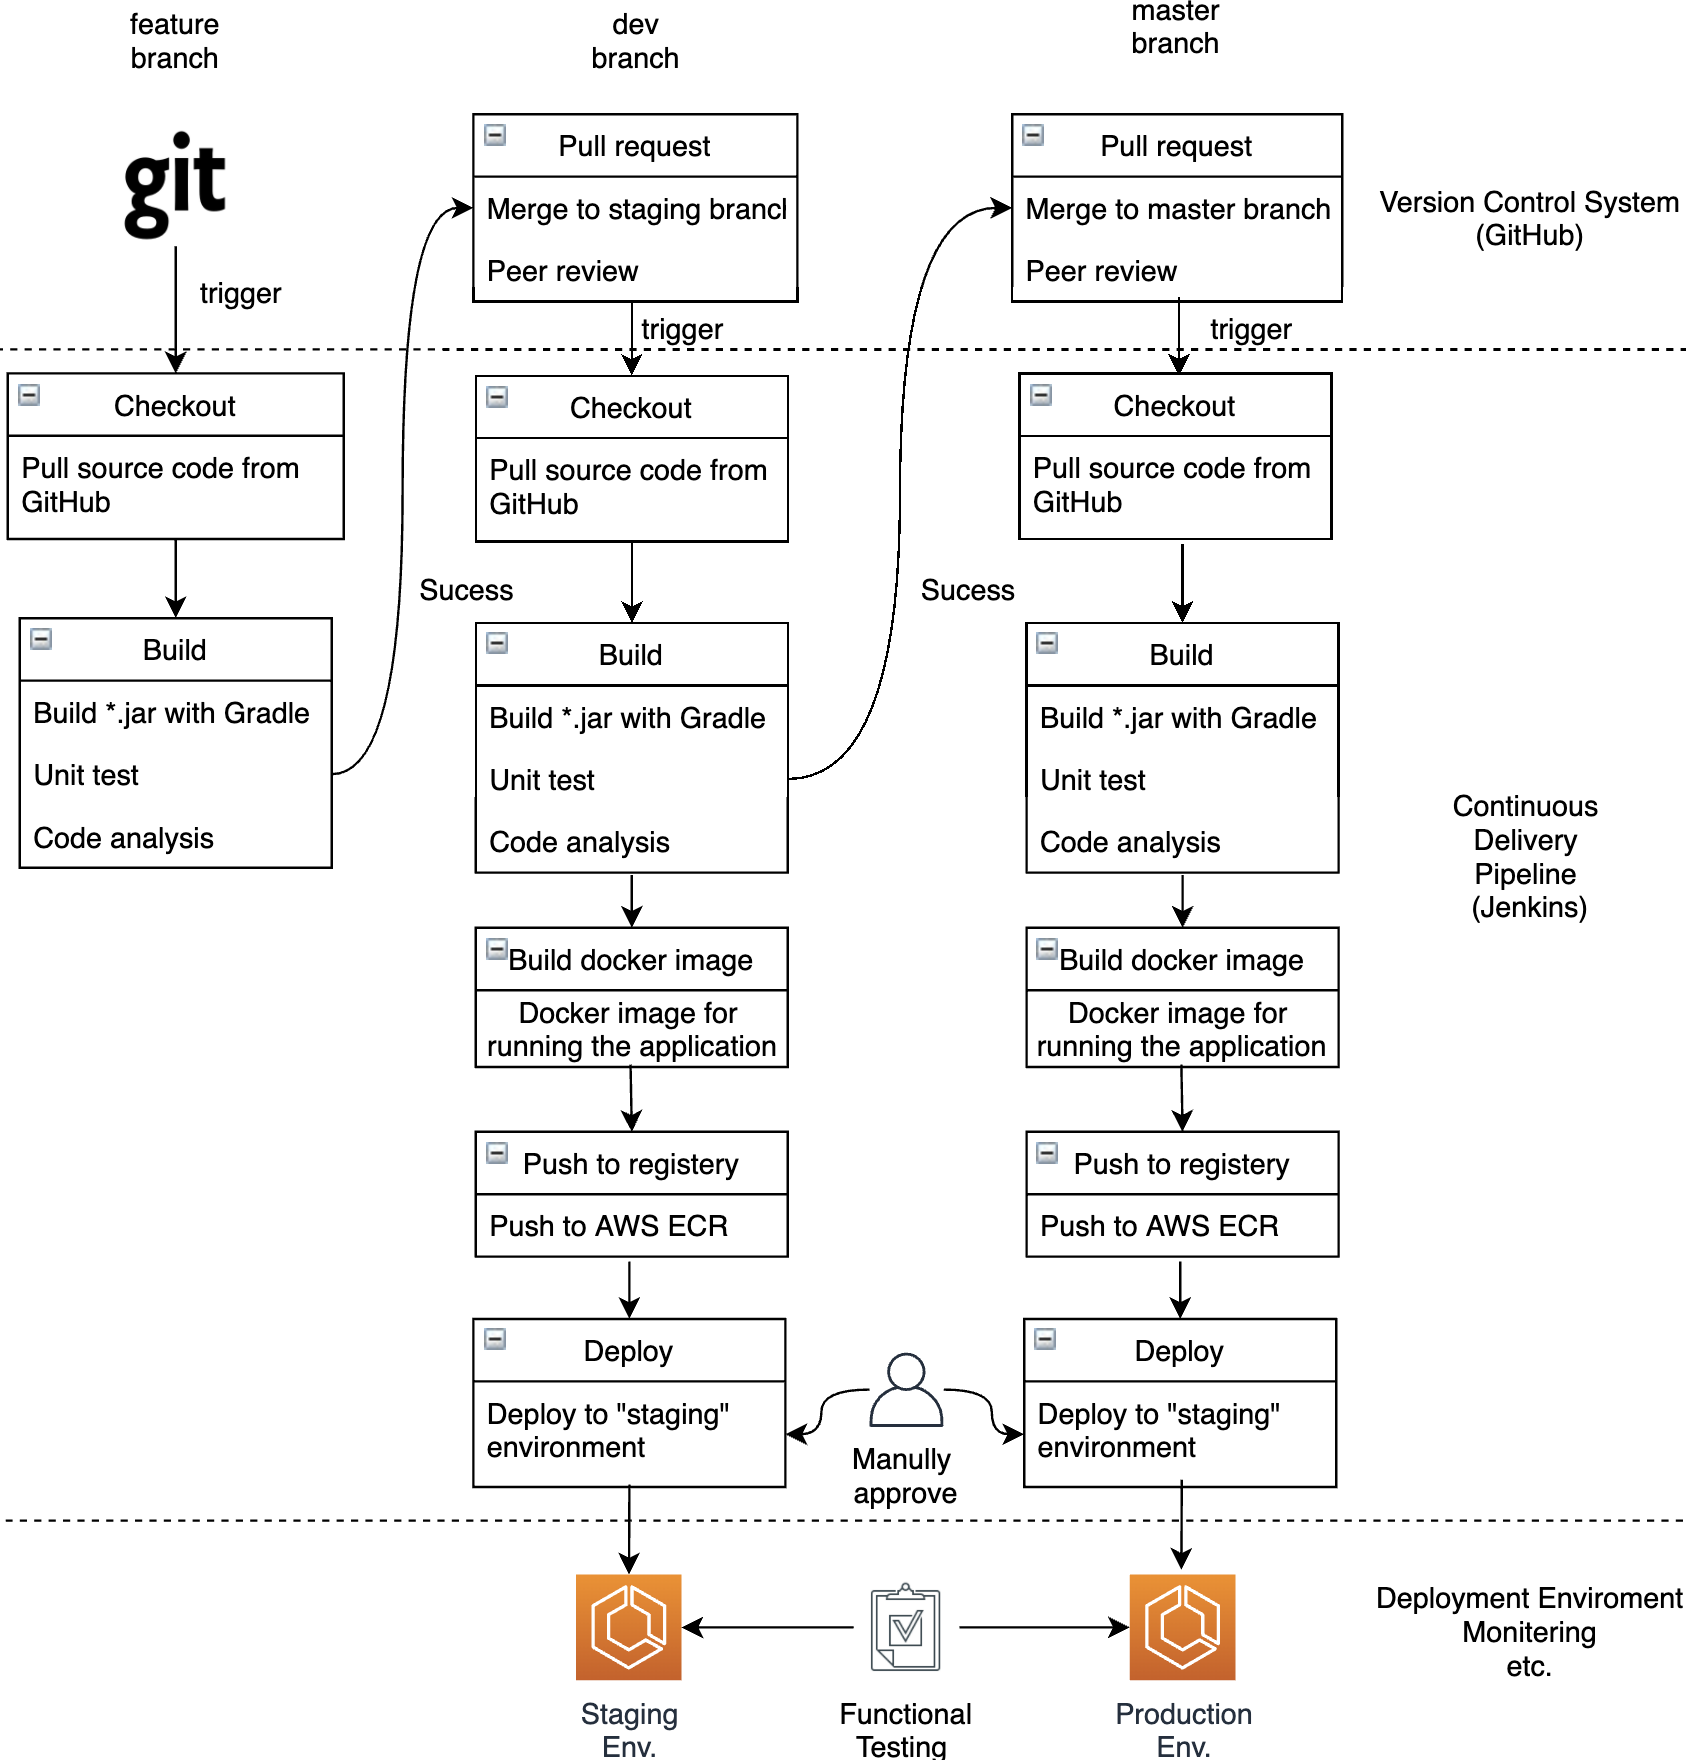
\includegraphics[width=0.99\textwidth]{pics/pipeline.png}
 \caption{The Workflow of Continuous Delivery Pipeline in Our DevOps Toolchain}
 \label{fig:pipeline}
\end{figure}
\paragraph[]{Workflow for Continuous Delivery}
Figure \ref{fig:pipeline} shows our proposed workflow of a project that goes through the continuous delivery pipeline.
We can see when the event on the feature branch triggers the pipeline, and it only runs through the first two stages. This is because according to the practices of continuous integration mentioned by us in \ref{CD} and by Martin Fowler in \cite{fowler2006continuous}, a developer should merge(the "integration" in continuous integration) his/her work couple times per day. Therefore the whole pipeline will run the code with this new feature at least several times a day. This already ensures the code could frequently be tested and deployed into the test environment. Thus, in the pipeline runs after the push to the feature branch, the further steps could be skipped. 
\par
 The developer only commits to the feature branch. The pipeline runs first two stages after a developer pushes local commits to Git. It first pulls the newly pushed code, and then build. In the build stage, the code first is analyzed, then we do unit testing to make sure the code could pass the test cases defined by the developer during development. In the end, the code will be built into Java ARchive file (.jar). The purpose of putting code analysis step first is that the code analysis will check syntax error and bugs. We want to make sure the code is runnable, and no syntax error before put it into the build. So we can reduce the cost by lowering pipeline running time if there is error exists in the code. 
\par
If no error returns after finishing all the above steps, the developer can open a pull request view the code change and ready to merge the code to the dev branch. Before the merge, the pull request needs to pass the code review by another developer. Code review is to make sure that the automated tests do not miss any bugs. After the code review passed, the reviewer or the developer him/herself merge the code to the dev branch.  
\par
After the code merged to the dev branch, the pipelines run again, this time it runs the whole pipeline. First, the pipeline executes the first two stages as in the feature branch. Now we have the Java ARchive file. The Java ARchive is an executable package of our Spring Boot application. Next step is to Dockerizing our application which generates the Docker image our application. Then we push the image to the Amazon Elastic Container Registry AWS (AWS ECR) for further use.
\par
\label{deploy}
The next step of the pipeline is deployment, the pipeline pull image in ECR that we pushed in the last stage, and then deploy it to the deployment environment in ECS with AWS CIL. The deployment strategy we are using is the rolling update. In the rolling update, we are gradually replacing instances in our deployment environment with the newer version of code.
\par
In the dev branch, we deploy the application to the staging environment. The deployment to staging environment should be automated. This is because the staging environment is only for testing and only visible within the team. 
In the staging environment, we will conduct API testing (last stage shows in Figure \ref{fig:overview}) for test if our deployed API works and if it works as expected. The test is being done by trigger a Lambda function. The Lambda function sends test HTTP request to the deployed endpoints, and verify if the HTTP response is correct. When the test is done, 
\begin{figure}[h]
     \centering
     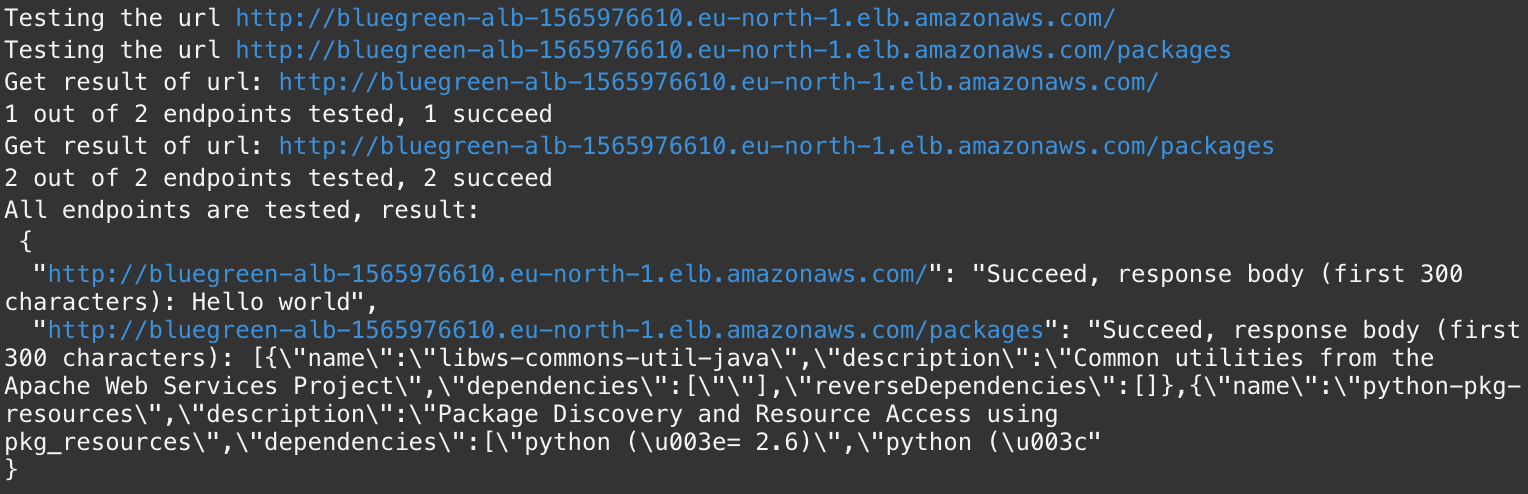
\includegraphics[width=0.98\textwidth]{pics/test_result.png}
     \caption{API Test Result (Jenkins log output)}
     \label{fig:test-result}
    \end{figure}
\par
If the deployed function passes the test, this shows the deployment works as expected and ready for the deployment. The developer could now open a pull request, merge code to master branch. The pipeline will runs again, and deploy the application to the production environment, which is visible to the customers.

\subsection{Deployment Environment}
\begin{figure}[h]
 \centering
 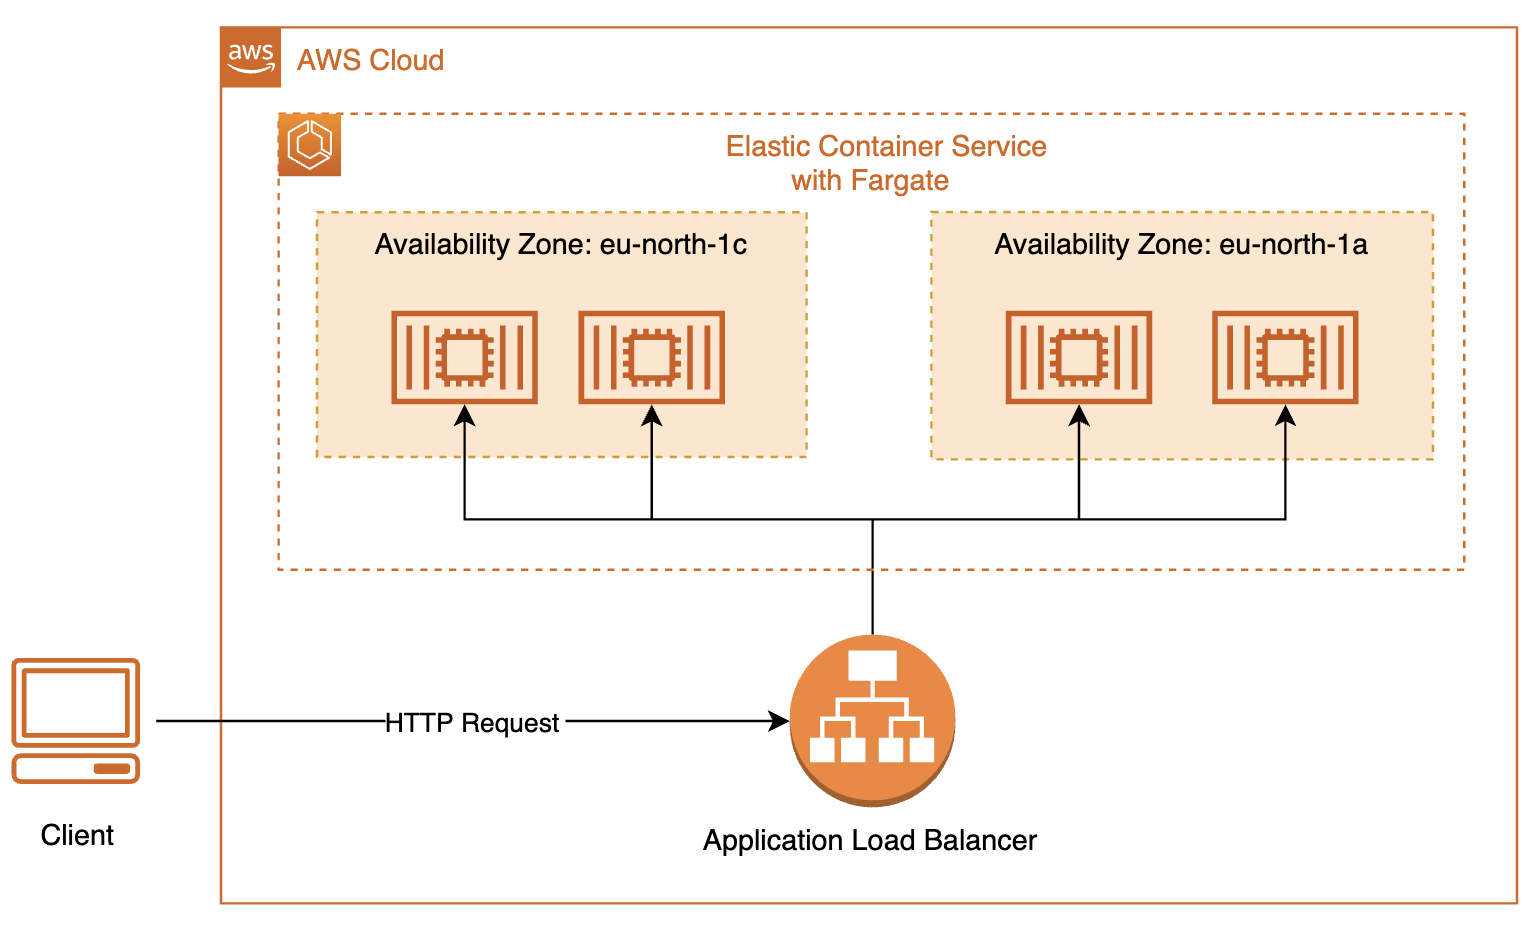
\includegraphics[width=0.99\textwidth]{pics/deploy.png}
 \caption{Deployment Environment}
 \label{fig:deploy}
\end{figure}
We create a simple deployment environment with AWS Elastic Container Service and Elastic Load Balancer. Same with Jenkins agents, we use Fargate to host our containerized case project. 
\par
AWS Fargate allow us to run our containerized application without having to manage servers, makes it easier for us to build a functionality complete DevOps toolchain implementation. We choose ECS over EKS (Elastic Kubernetes Service) is because ECS is free of charge while EKS charges extra for the runtime of the cluster. Compared with EKS, ECS also provides better integration with other AWS services, such as with AWS DevOps toolchain, and AWS CloudWatch monitoring.
\par
Figure \ref{fig:deploy}
shows our deployment architecture. The deployment region in Stockholm(EU-north-1). The Fargate instances in ECS cluster are automated scaled according to the number of incoming requests. 
To improve the availably of the product, we deploy the case project into two different availability zones within the region. 
When one availability zone is down, the load balancer can route the request makes sure the request can still reach the healthy availability zone. Besides the availability improvement, the load balancer also distributes incoming requests across Fargate instances which maximizing the resources rate within our ECS cluster.
% During deployment, we use Martin Fowler's blue and green deployment strategy \cite{fowler2010bluegreendeployment}, which is natively supported by ECS. This means when a new deployment comes, the older version will continue serving until the newer version reaches the stable status. This could significantly reduce the downtime in the deployment. 
% \subsection{Smoke Testing}
% Testing is an implement component within the DevOps pipeline
% In this section, we further discuss the smoke testing that we mentioned in the \ref{deploy}.
\subsection{Monitoring}
Monitoring is one of the important components in the DevOps toolchain. Different from testing, which usually integrated with the continuous delivery pipeline, the monitoring is independent of the pipeline. Usually, monitoring does not act as one step within the continuous delivery pipeline but as an independent component.
\par
In Chapter 3, we introduced AWS CloudWatch as one of the serverless services in AWS. In our toolchain, we will use it as the tool for monitoring the cloud infrastructure. With Cloudwatch, we not only can get the realtime log from our deployed container in the ECS but also the quantitative data, for example, memory utilization and network i/o, the monitoring dashboard can seem at figure \ref{fig:monitoring}
\begin{figure}[!tbp]
     \centering
     \begin{minipage}[b]{0.47\textwidth}
       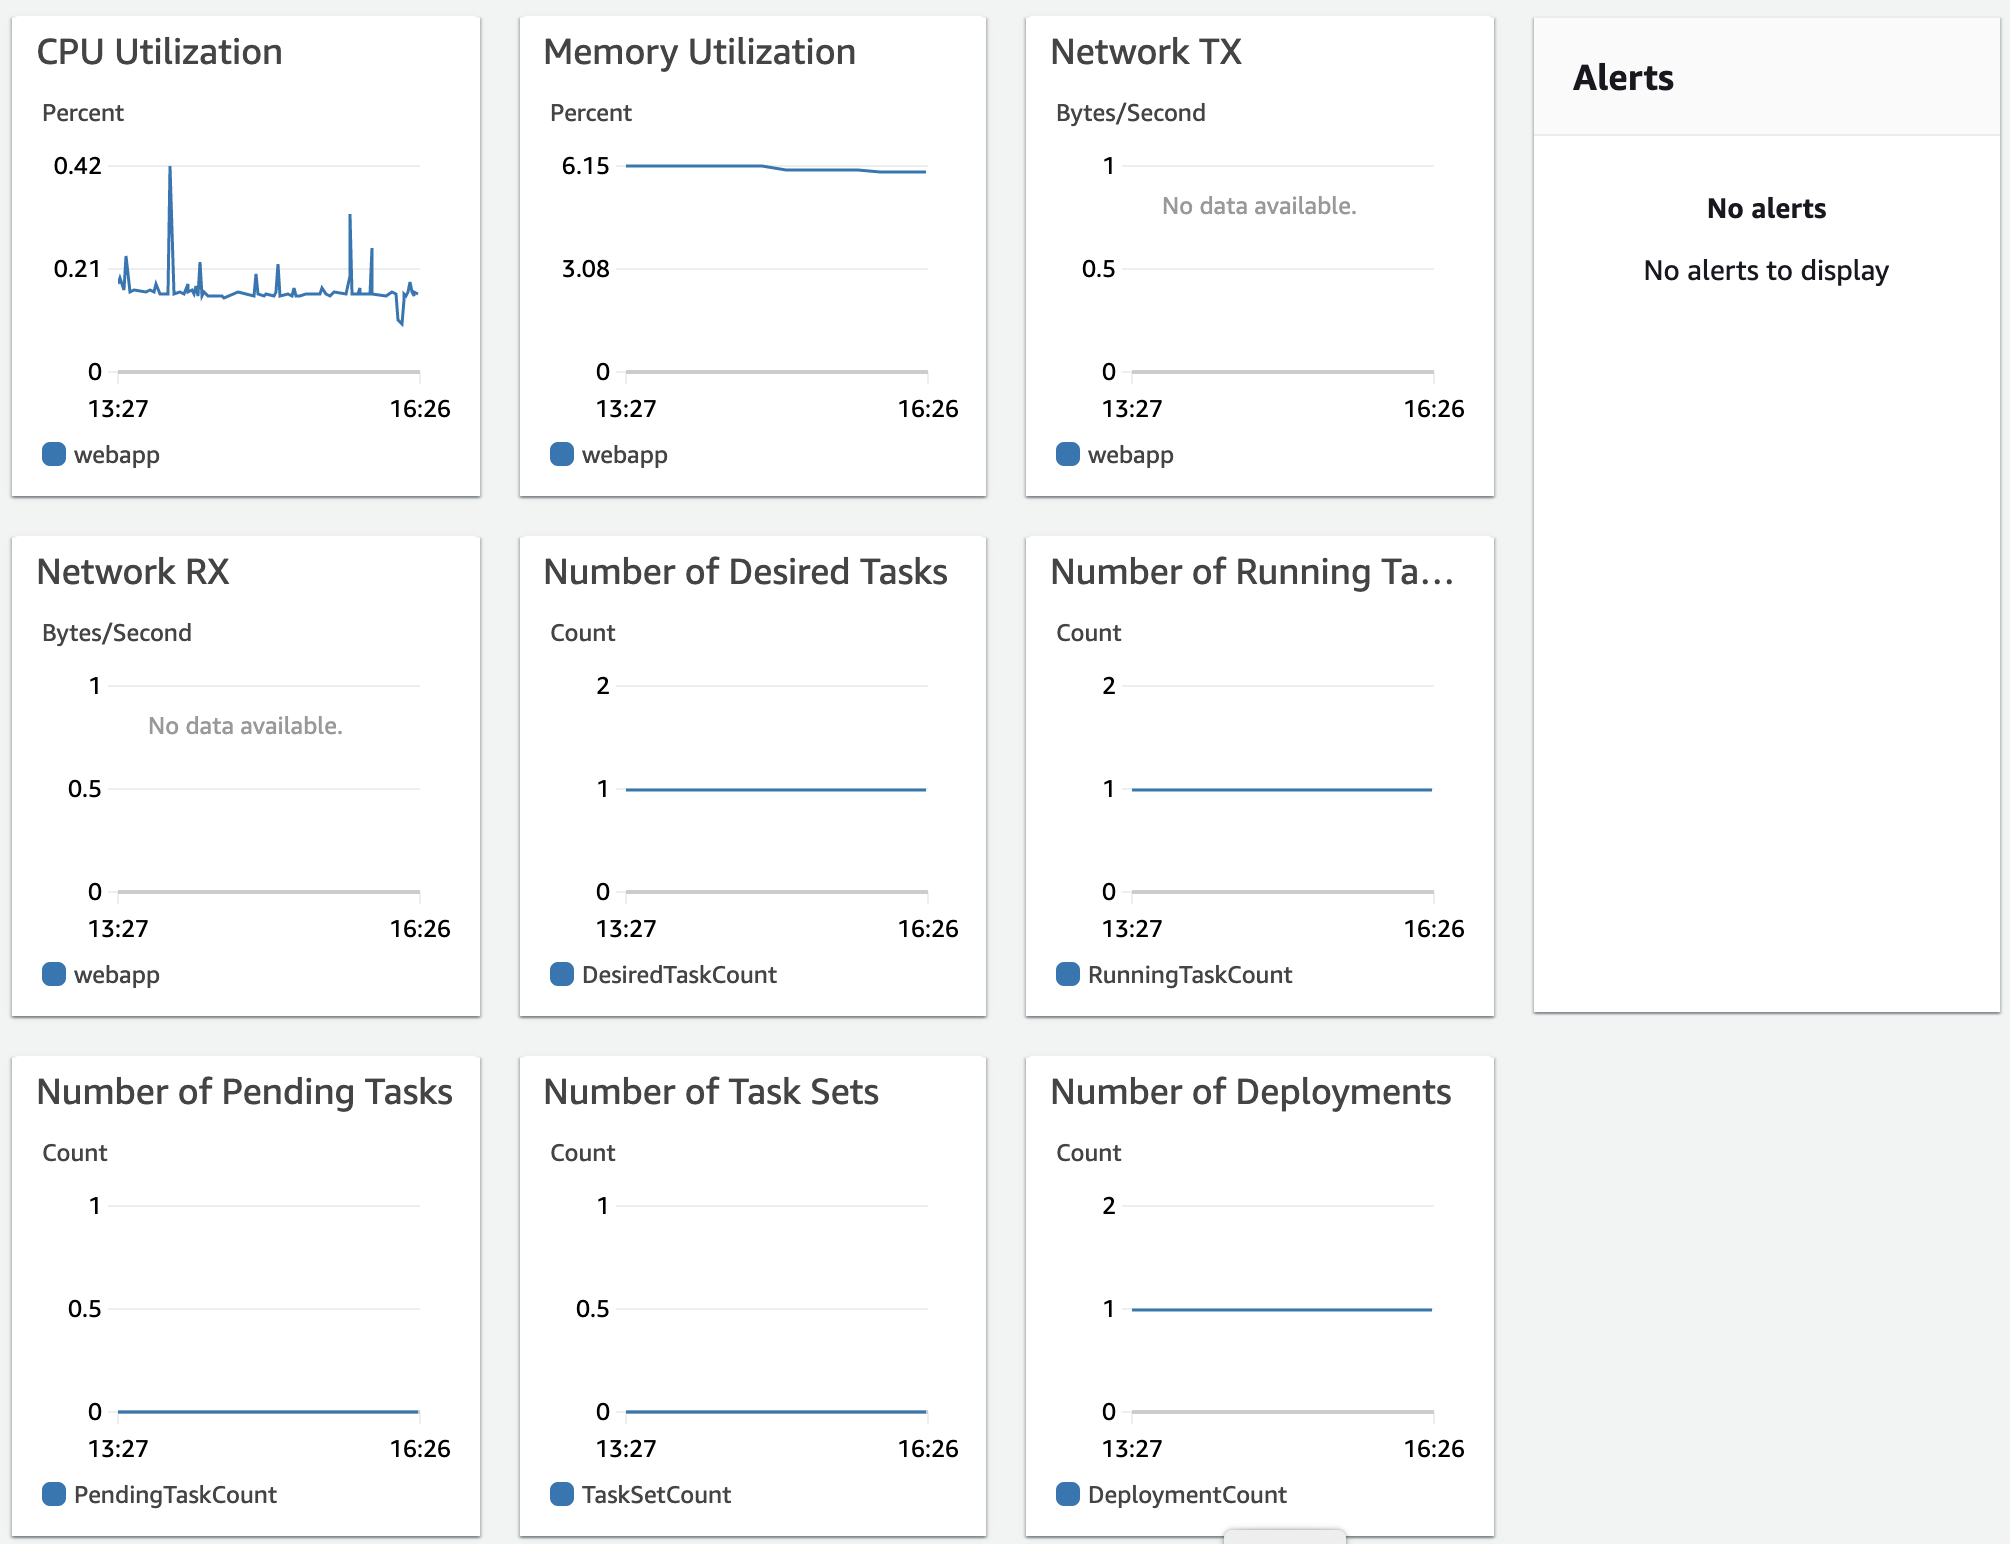
\includegraphics[width=\textwidth]{pics/monitoring.png}
     \end{minipage}
     \hfill
     \begin{minipage}[b]{0.50\textwidth}
       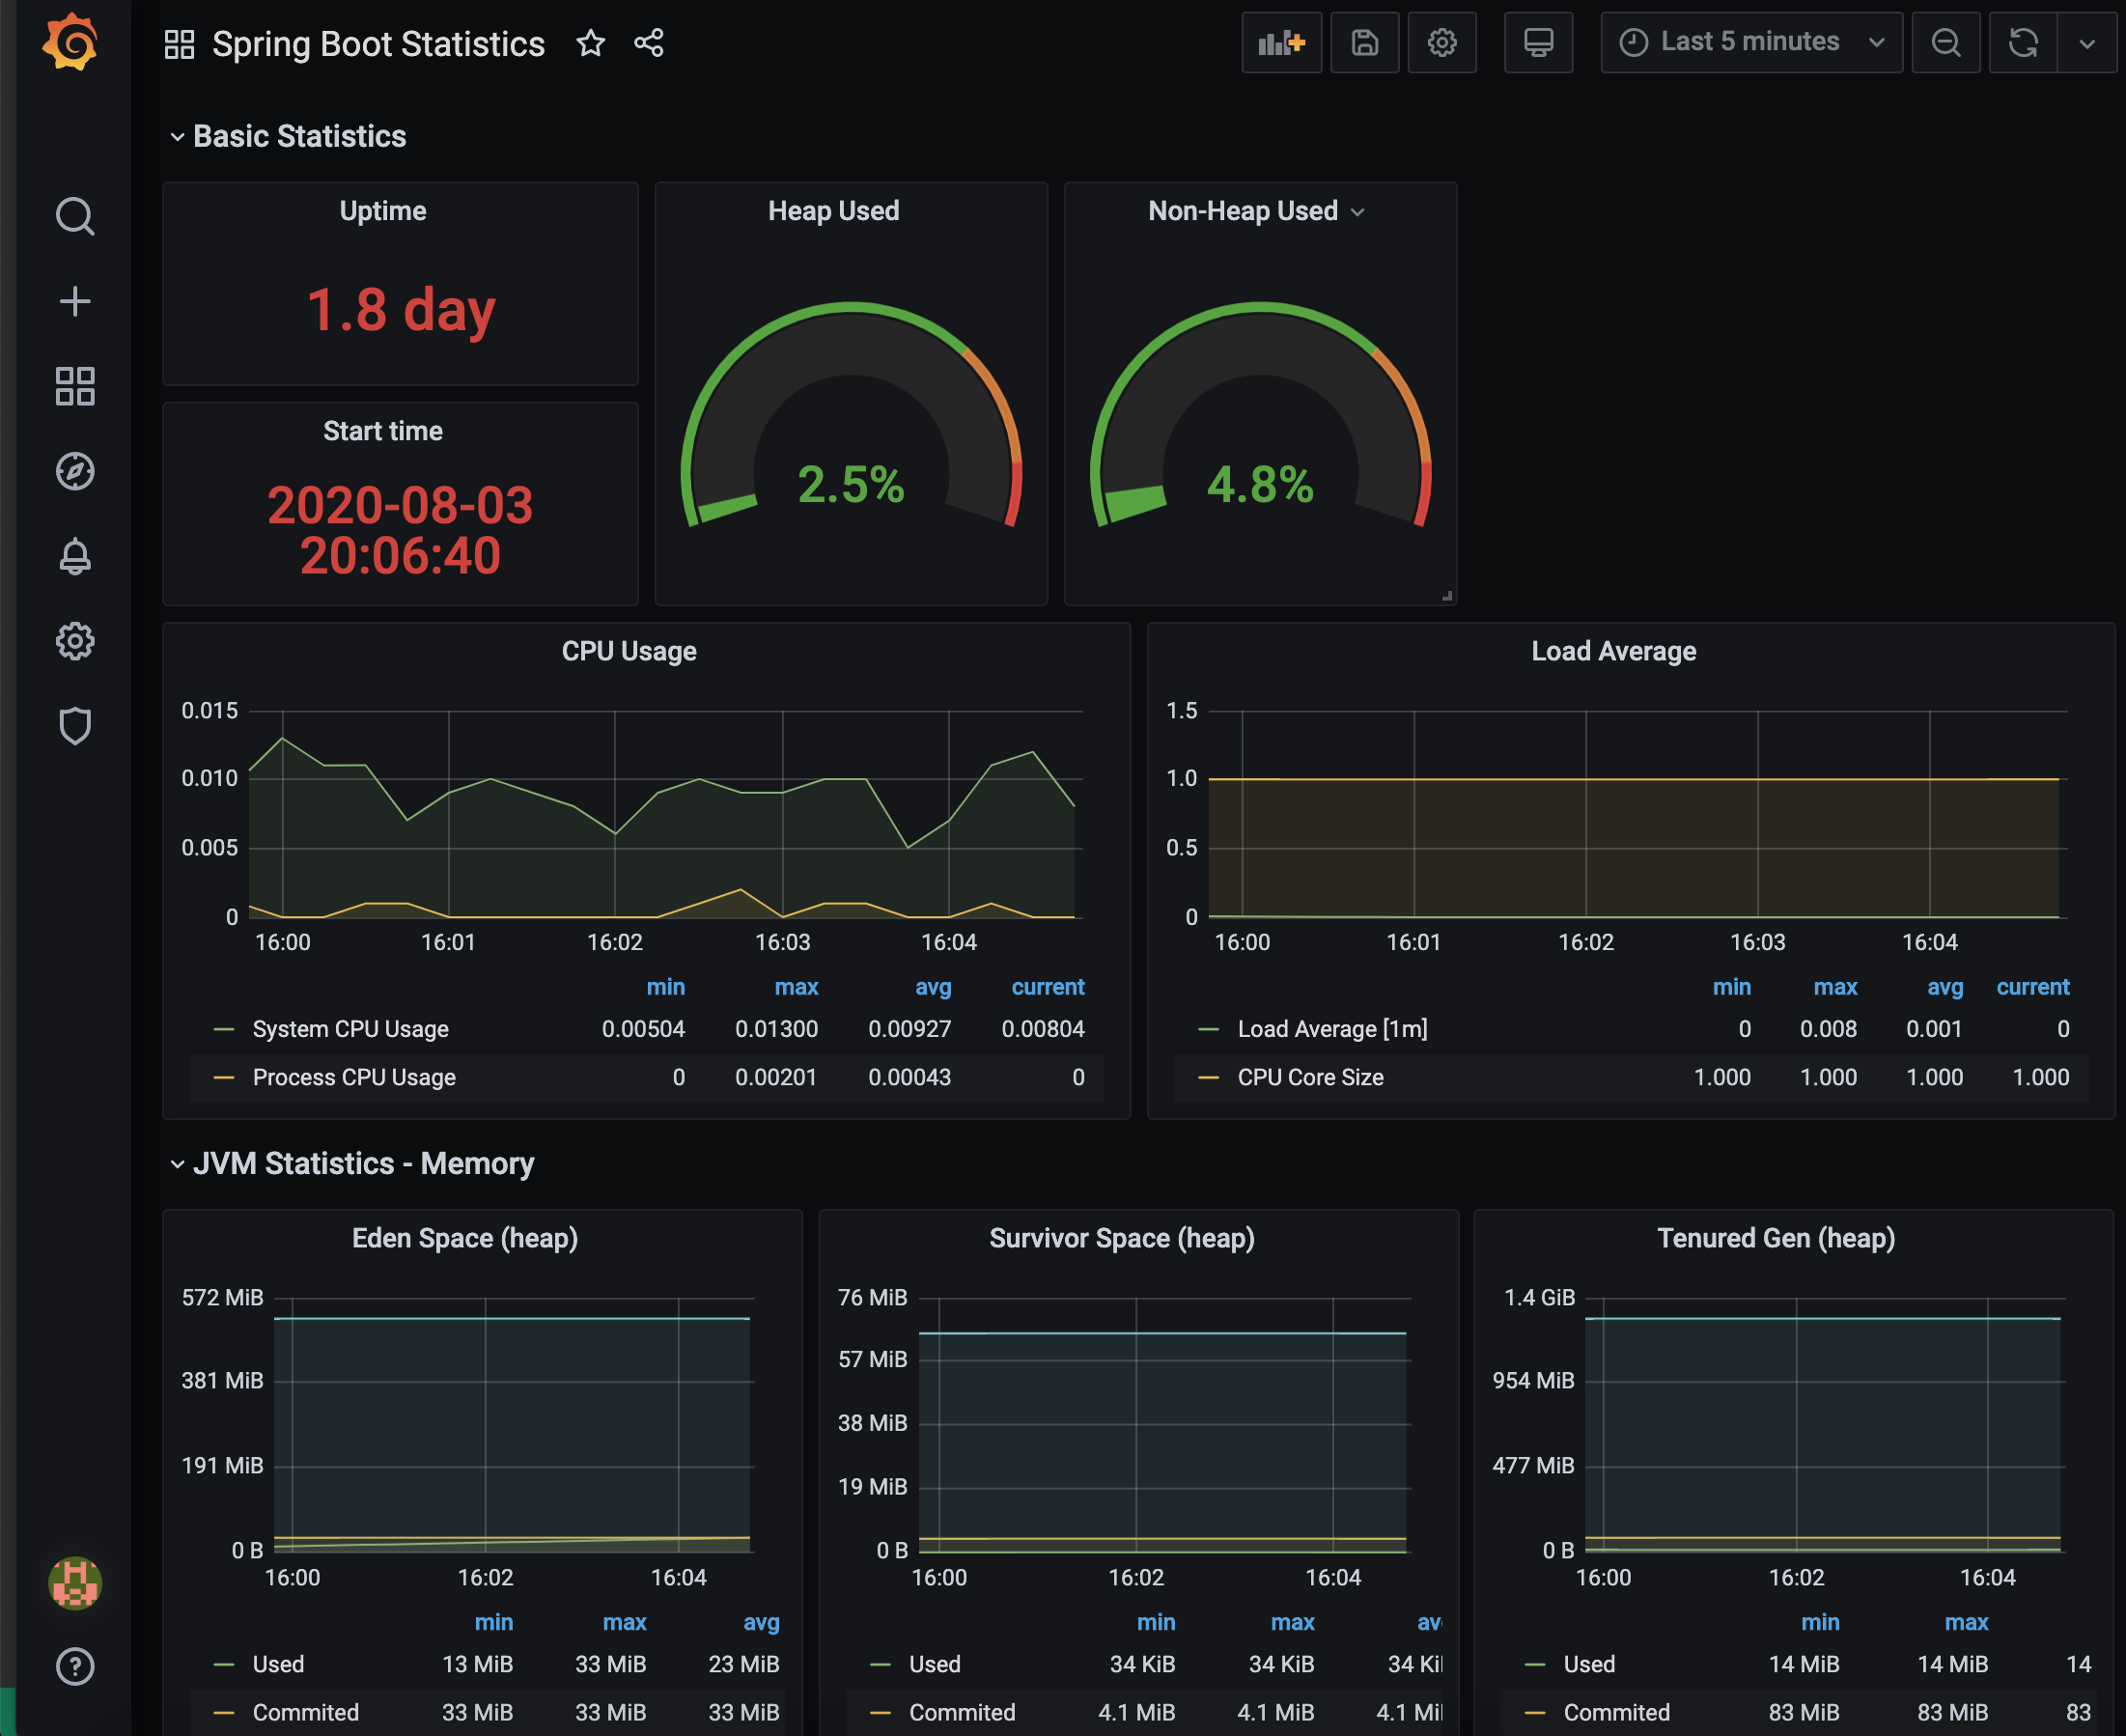
\includegraphics[width=\textwidth]{pics/grafana.png}
     \end{minipage}
     \label{fig:monitoring}
     \caption{The Monitoring Dashboard of CloudWatch (Left) and Grafana (Right)}
   \end{figure}
\par
In the last paragraph of section 4.2.2, we mentioned that the CloudWatch is not capable to monitor what happens inside the application framework, in our case, Spring boot. Thus, we use Prometheus to gather the metrics within our Spring Boot application. Prometheus gather the realtime metrics with the help of Micrometer plugin of Spring boot. Micrometer exports all numeric metrics in realtime, these metrics includes, JVM statistics, CPU/RAM utilization, number of request to each API endpoint and the user's self-defined metrics within Java code. Prometheus records these metrics every second, and save the metrics in time series to Database. In addition to Prometheus, we use Grafana for read the metrics from Prometheus and display the metrics on the dashboard.
\par
Another service we introduced in Chapter 3 is AWS lambda. It is the most important serverless service in AWS. We also discussed how could it be used in our DevOps toolchain in which monitoring is one of the use cases. In our monitoring system, AWS lambda is used as an extension for CloudWatch, and we use it for 2 cases.
\paragraph[]{Auto-Scaling the ECS Cluster with Custom Alarm in Cloudwatch}
As we mentioned in \ref{fig:deploy} Deployment Environment, The deployment could be auto-scaled by defining the auto-scaling policy within the ECS cluster. However, the scaling policy is not flexible enough; it only based on thresholds on certain metrics such as CPU utilization and memory utilization. Such auto-scaling in practice is: When the watched resources utilization is above/below a certain threshold, an alarm in Cloudwatch will be triggered. The alarm will further trigger the scaling event if the scaling policy was being set before.
\par
Nevertheless, in real-life development, many projects are microservices architecture, rather than homogeneous architecture as we have in the case project. According to Luca Tiozzo's article \cite{AWSECSho47:online}, this means some service (container instance in ECS) could be CPU intensive while the others might be RAM intensive. In such a situation, with Cloudwatch alarm based scaling, we need two groups of alarm watching RAM and CPU, respectively. Nevertheless, the problem is, when the ECS cluster lack of CPU resource but lack of RAM recourse, the CPU alarm is triggered then the ECS scaled up. Now the ECS cluster has enough CPU recourse, but it may have too much RAM resource so that it triggers the scale-in alarm in RAM. So the cluster will scale in again. This will cause the cluster to keep scaling up and back without finding and suitable size.
\par
A good practice solves the problem is to use a single group of alarm that only triggered by single metrics. We can set an AWS lambda function that read different metrics and then aggregate it to a single custom metric. The software team determines the threshold and metrics according to the deployed project. Once the aggregated metric reach the threshold, the lambda function triggers an alarm that can trigger the scaling of ECS cluster. 
\paragraph[]{Custom Project-Specific Metrics}
The second application scenario is related to the first one. The Cloudwatch has support on recourse utilization metrics. However, some metrics are project-specific and not related to resources utilization and performance. For example, the number of successful payment has been made in a payment service. In such a case, Lambda could fill the gap within the scope of CloudWatch. The team could set up a Lambda function which gets the number by monitoring the log with PutMetricData provided by CloudWatch. This Lambda can further forward the metrics to metrics analysis and visualization platform, for example, Grafana \footnote{https://grafana.com/grafana/} to give the management team an overview of the KPIs.
\section{Design of Integrated Serverless DevOps Toolchain}
AWS provides a set of serverless DevOps tools which could help us build a completely serverless DevOps toolchain. We introduced these tools in Chapter 3. In the section, we introduce the design of Serverless toolchain based on DevOps tools of AWS. A certain part of the toolchain is the same with the non-integrated DevOps toolchain that introduced in the last section. Therefore we will not introduce these components again. Rather we only focus on how do we make use AWS DevOps toolchain. Figure \ref{fig:codepipeline} shows the general workflow of a project delivered by our integrated DevOps toolchain.
\begin{figure}[h]
 \centering
 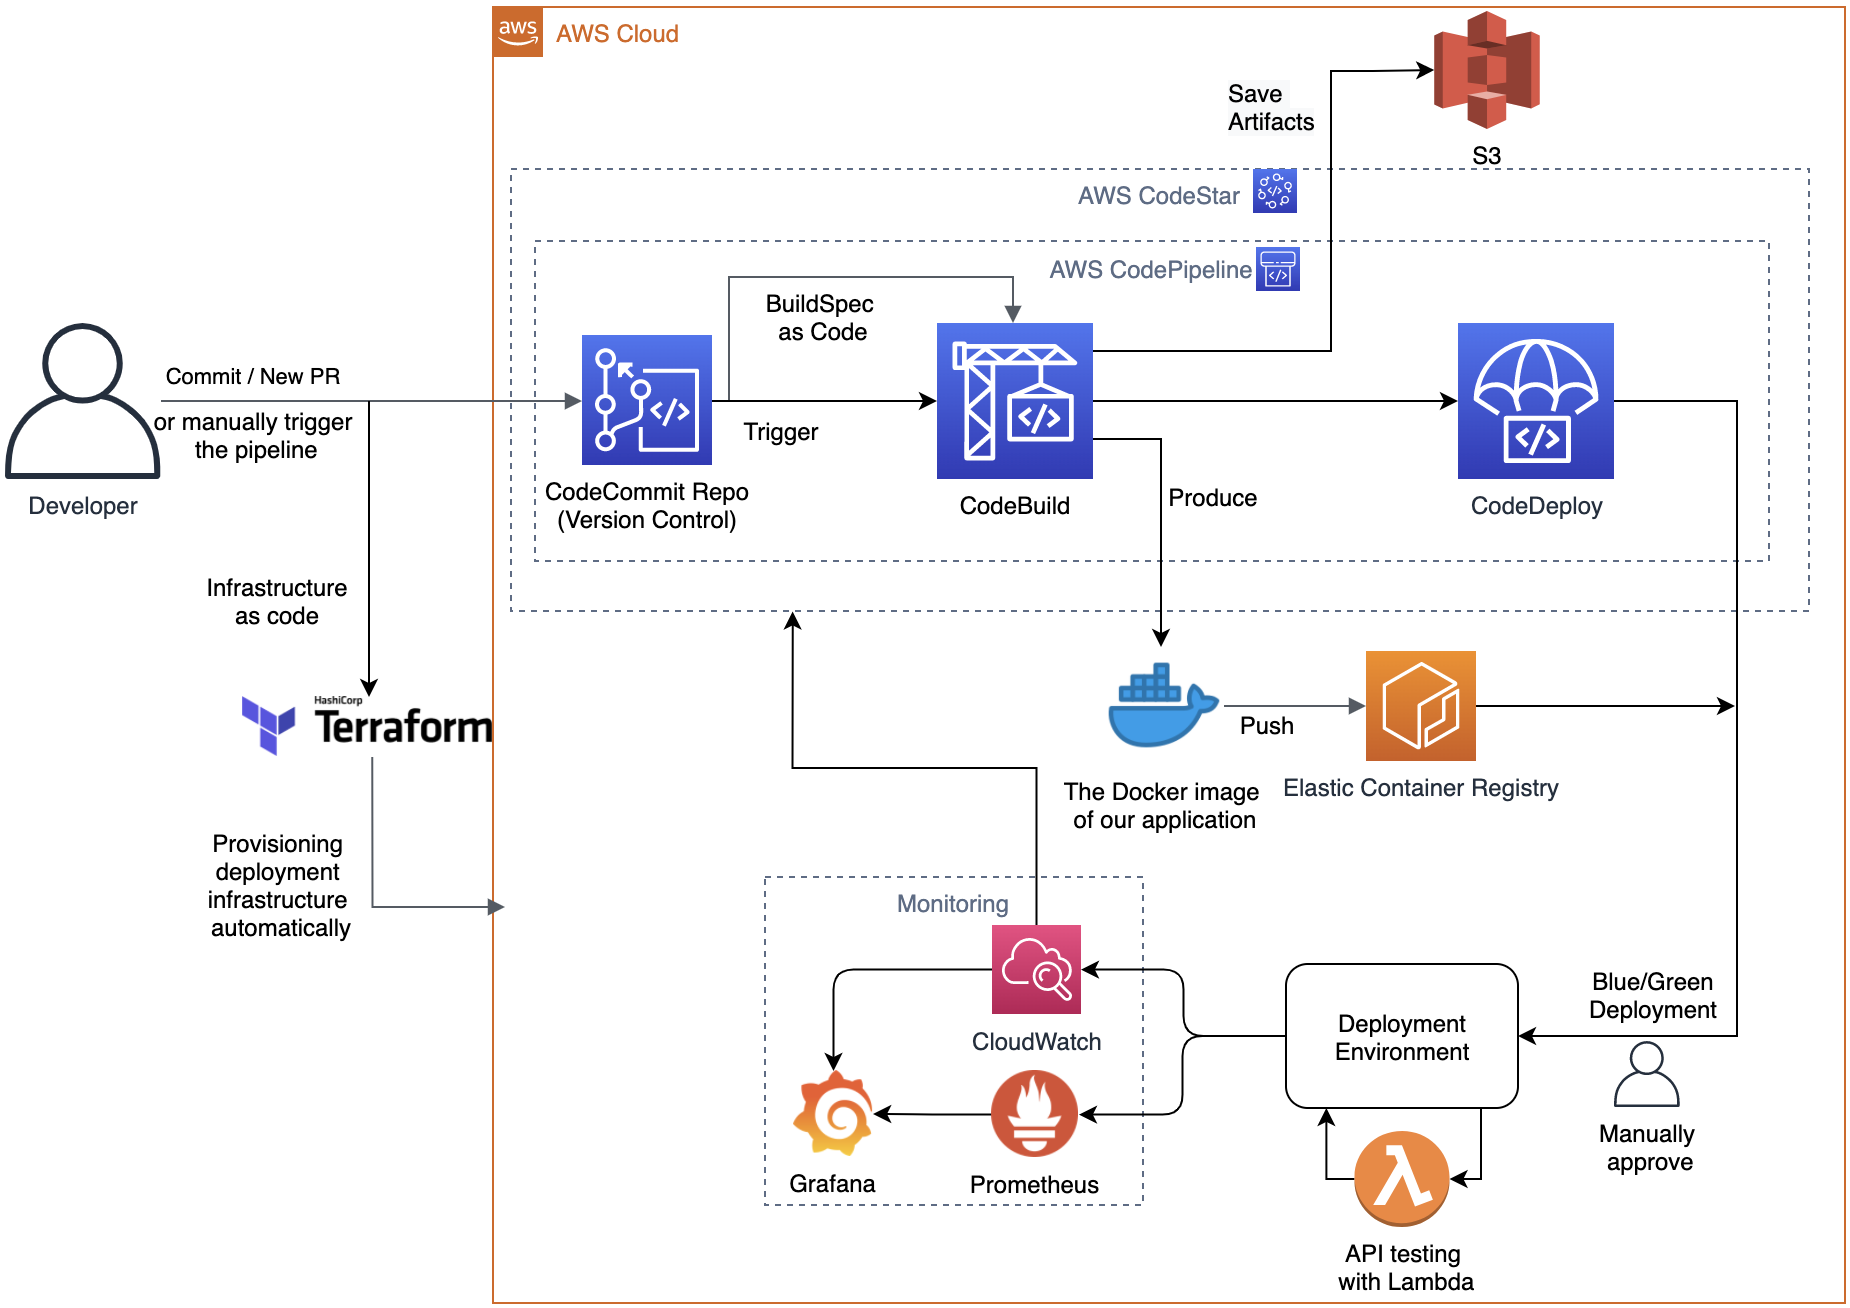
\includegraphics[width=0.90\textwidth]{pics/codepipeline.png}
 \caption{Integrated Serverless DevOps Toolchain}
 \label{fig:codepipeline}
\end{figure}
\subsection{Continuous Delivery Pipeline with AWS CodePipeline}
The workflow of our continuous delivery pipeline is the same as the pipeline in \ref{CD}. Instead of Jenkins, which is server-based, we build the pipeline with AWS CodePipeline. Figure \ref{fig:codepipeline} shows the activity within the CodePipeline in a single graph. Different from Jenkins who can do the whole continuous delivery process solely with the help of plugins, the CodePipeline just provides a platform which the development team can configure a workflow with AWS DevOps tools or other third-party tools. 
\par
Same within the non-integrated version, we used GitHub as the version control system, and it has the same role as it has in the non-integrated toolchain. Although AWS also provides version control solution which is CodeCommit. It still lacks the functionality of collaboration compared with GitHub. Also, GitHub is already a serverless solution with good integration with AWS DevOps tools, so we do not need to change our version control system away from GitHub. 
\par
In the next step, we are using AWS CodeBuild, which we introduced in Chapter 3. AWS CodeBuild does the same procedure as in Jenkins pipeline. It does code analysis, unit test and builds the Java application with Gradle, build the Docker image of the application and push to the ECR. Different, the cloud deployment deploys our application to ECS with Blue-and-green deployment strategy.
\par
The implementation of continuous delivery in CodePipeline is straightforward compared with Jenkins. In Jenkins, without the help of the plugin, the pipeline workflow can only be defined by groovy code, while CodePipeline natively provides a graphical user interface for workflow modelling. In our implementation, we just simply add each step with the graphical interfaces in CodePipeline.
\begin{figure}[h]
 \centering
 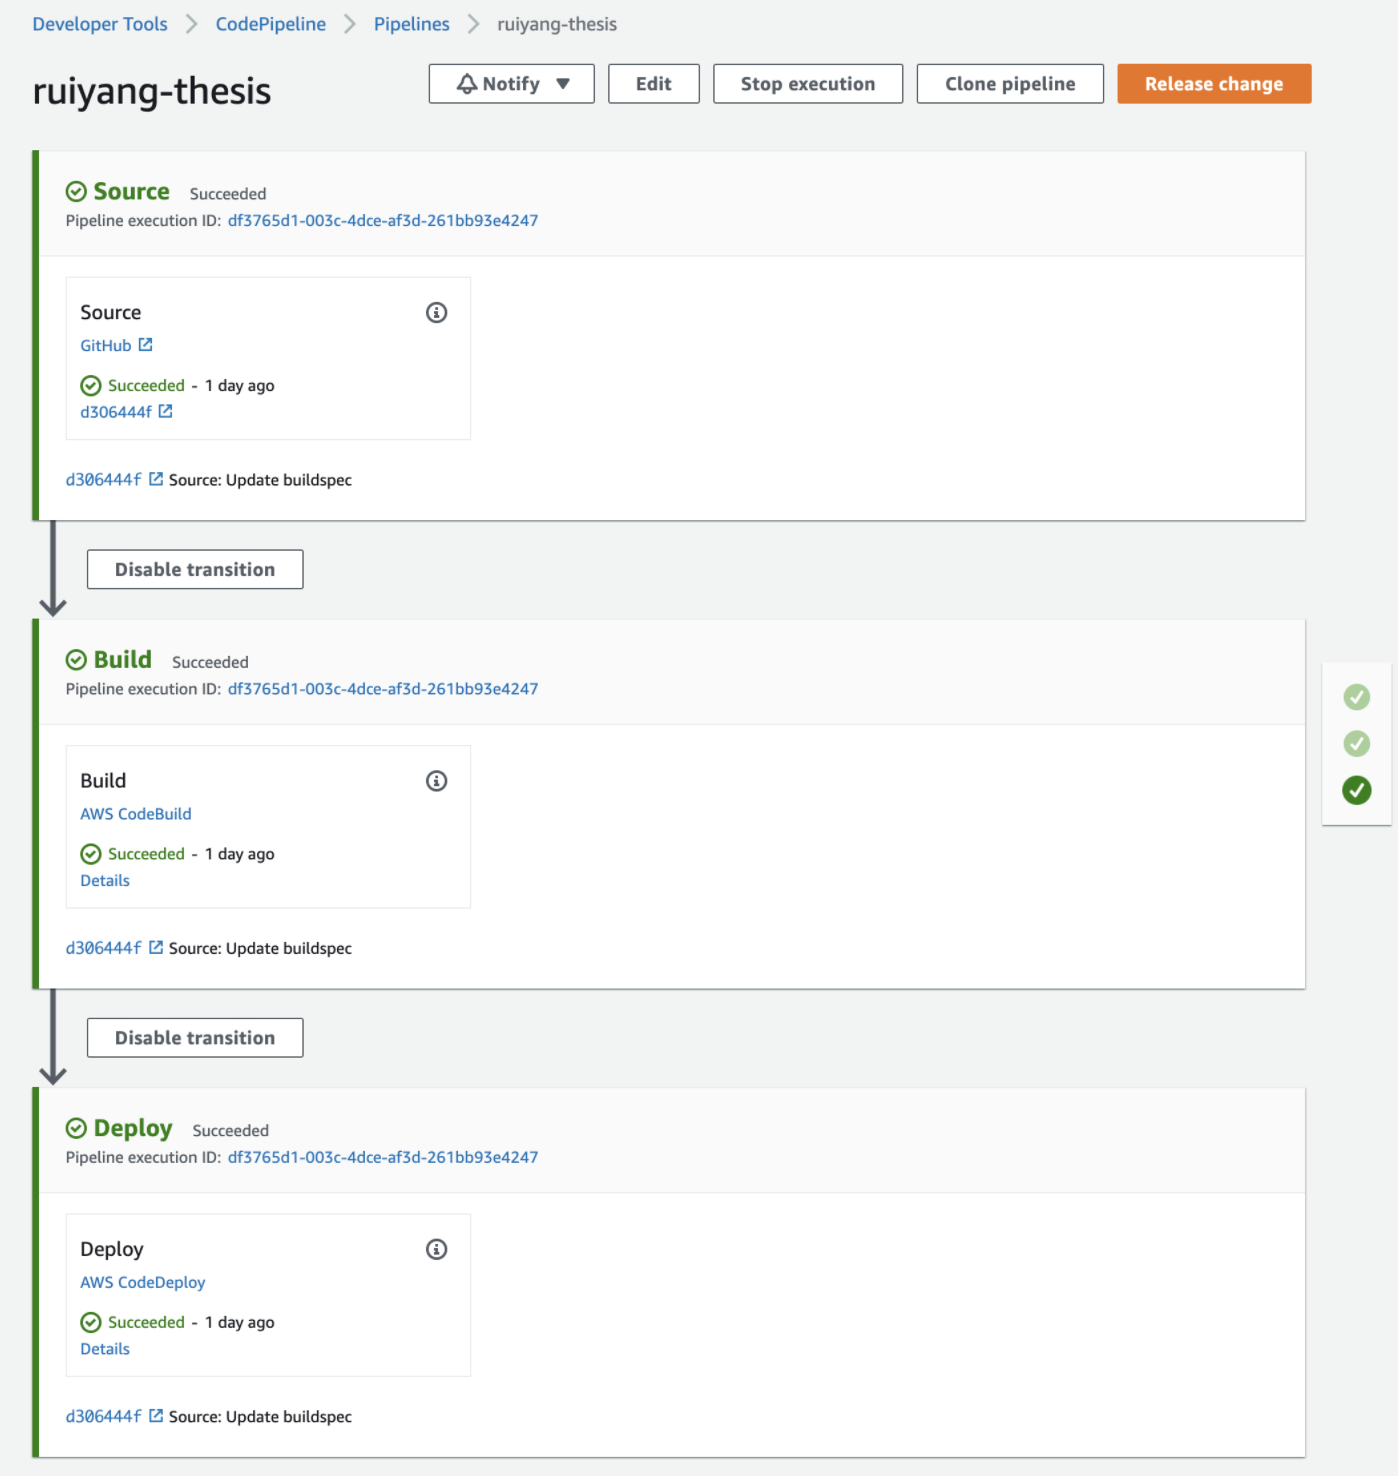
\includegraphics[width=0.75\textwidth]{pics/cp-interface.png}
 \caption{Our Workflow in CodePipeline}
 \label{fig:cp-edit}
\end{figure}
\subsection{Build and Test with AWS CodeBuild}
Same with the design of our Jenkins pipeline, AWS CodeBuild also executes the build within Docker container. The image of the Docker container provided by AWS already contains environment for the build of different programming languages. It also includes the Java environment and Gradle which needed by our case project. Therefore we could save time in setting up the pipeline since we do not need to define the Docker image for the build by ourself.
\par
As we mentioned in 4.3.1, the process within CodeBuild is the same as we have in Jenkins before the stage "Deploy". We will not describe the process again here. Same with Jenkins, the workflow of CodeBuild is defined in a YAML configuration file. The only difference in term of build workflow CodeBuild is that we store the build artifact to S3, the build artifact is the configuration file defines the deployment configuration in CodeDeploy. This is because CodeDeploy requires the deployment configuration from the step before it to run automatically.
\subsection{Blue/Green Deployment with AWS CodeDeploy}
One of the advantages of AWS DevOps tools is good integration with other AWS services. During the design and implementation of our toolchain, this advantage shows in the deployment to ECS with CodeDeploy.
\par
In Jenkins, there is a lack of specific plugin that helps us deploy the project into ECS or EKS. Thus we have to deploy our project to ECS with AWS command-line interface(CIL). The problem with AWS CIL is that it only supports the most basic deployment strategy, which is rolling update deployment. The rolling deployment strategy is to replace the old code running on the instances with new code gradually, instance by instance. 
\begin{figure}[h]
 \centering
 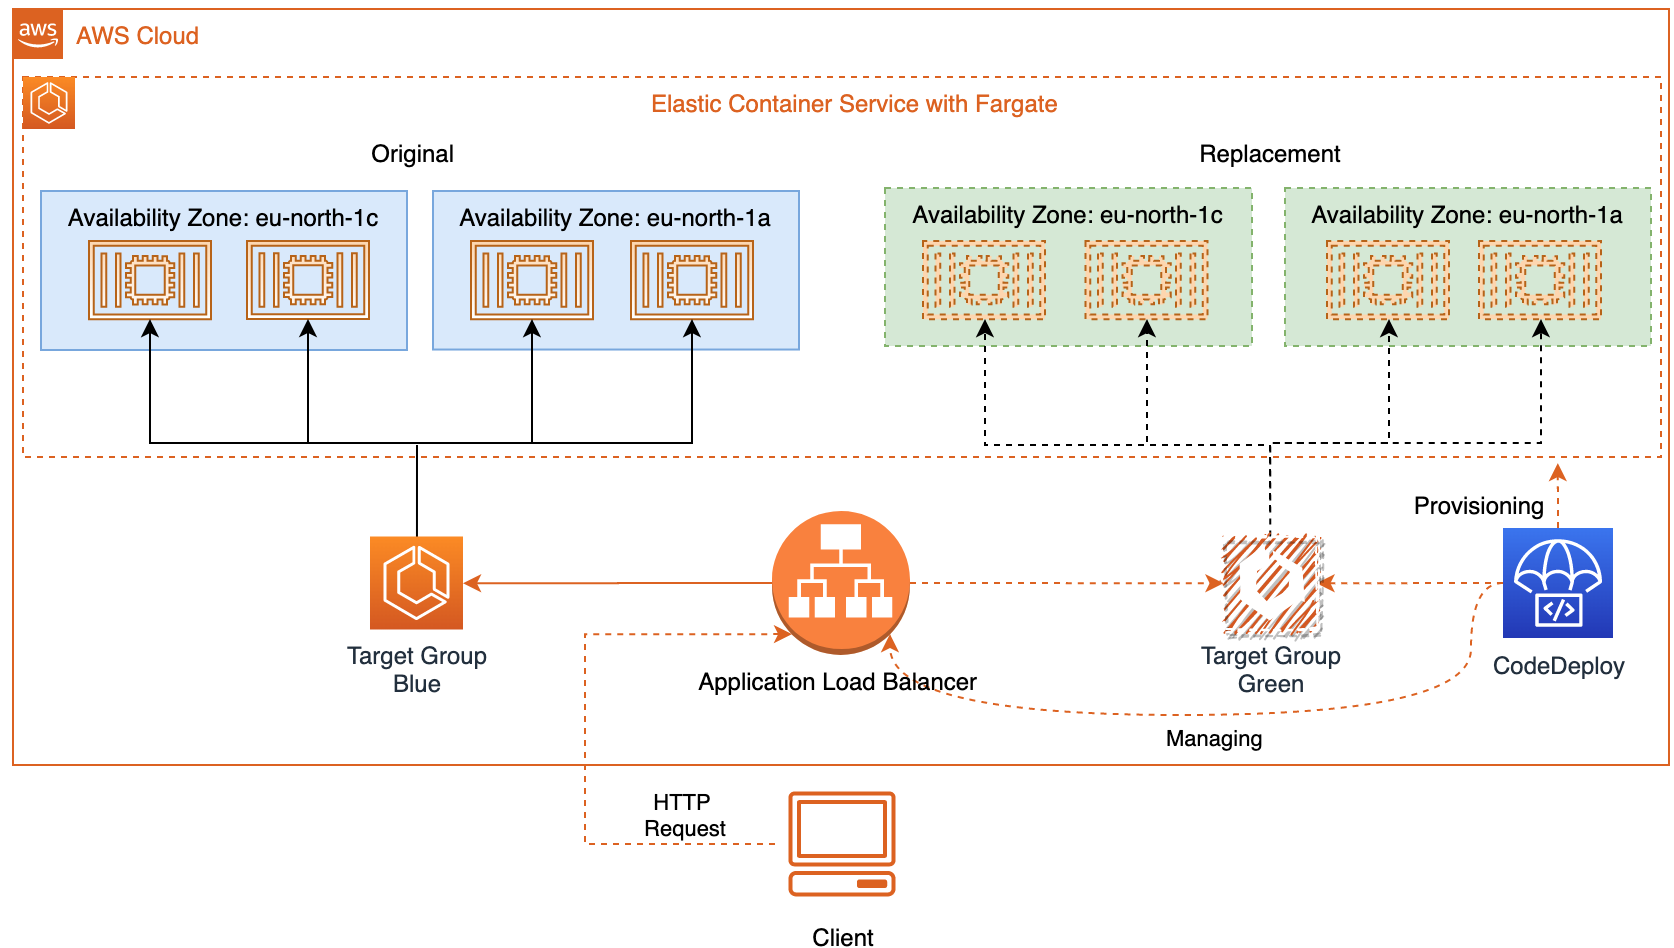
\includegraphics[width=0.99\textwidth]{pics/bg.png}
 \caption{Blue and Green Deployment for Our Deployment Solution}
 \label{fig:bg}
\end{figure}
\par
In real-life production, the team would like to make sure the deployment is reliable with minimized downtime. Thus the safety is highly valued in deployment strategy. In answering this need, a strategy called blue/green deployment, which is now widely used in the industry. AWS CodeDeploy natively supports the blue/green strategy.
A blue/green deployment is a deployment strategy that requires two sets of totally identical deployment environment that runs the new and original version of code respectively, while the load balancer is gradually routing more incoming requests to the environment that runs the newer version of code. 
\par
Figure \ref{fig:bg} shows the visualisation of blue/green deployment. It also shows our design on how to implement blue/green deployment with CodeDeploy (shown before in Figure \ref{fig:deploy}). CodeDeploy controls routing policy within the load balancer. When new deployment comes, CodeDeploy does the following steps:
\begin{itemize}
 \item Provisioning new identical deployment environment (replacement environment) and deploy a newer version of code on it. In ECS, the deployment is called "task set".
 \item Control the load balancer, rerouteing incoming traffic gradually to replacement ECS task set. We set the rerouteing rule as 10\% per minuets. We do not rerouteing all traffic at once to ensure the service will not fully down if the new deployed task set not works properly. This minimizes the downtime of our deployment.
 \item Wait for 5 minutes after rerouteing is done. During the rerouteing and this 5 minutes, the load balancer keeps doing the health check to the new deployment by sending a request to the health check API endpoint. CodeDeploy read the health status from the load balancer. If the replacement tasks set is un-healthy, CodeDeploy does rollback by rerouteing incoming traffic back to origin tasks set.
 \item If the new deployment is still healthy after 5 minutes of waiting time, CodeDeploy terminates the origin tasks set. Now the whole deploy process is done.
\end{itemize}
Compare with the rolling update we are using in Jenkins pipeline, the better safety of blue/green deployment reflected at, when the error happens with a newer version of code, we can immediately roll back to the last version by switching the rerouteing to Blue \cite{UsingBlu65:online} without redeploying the previous version. Under the same circumstance, the rollback with the rolling update is nevertheless taking a too long time, since we have to replace the already deployed code to the previous version. This could cause longer downtime of the server. 
\begin{figure}[h]
 \centering
 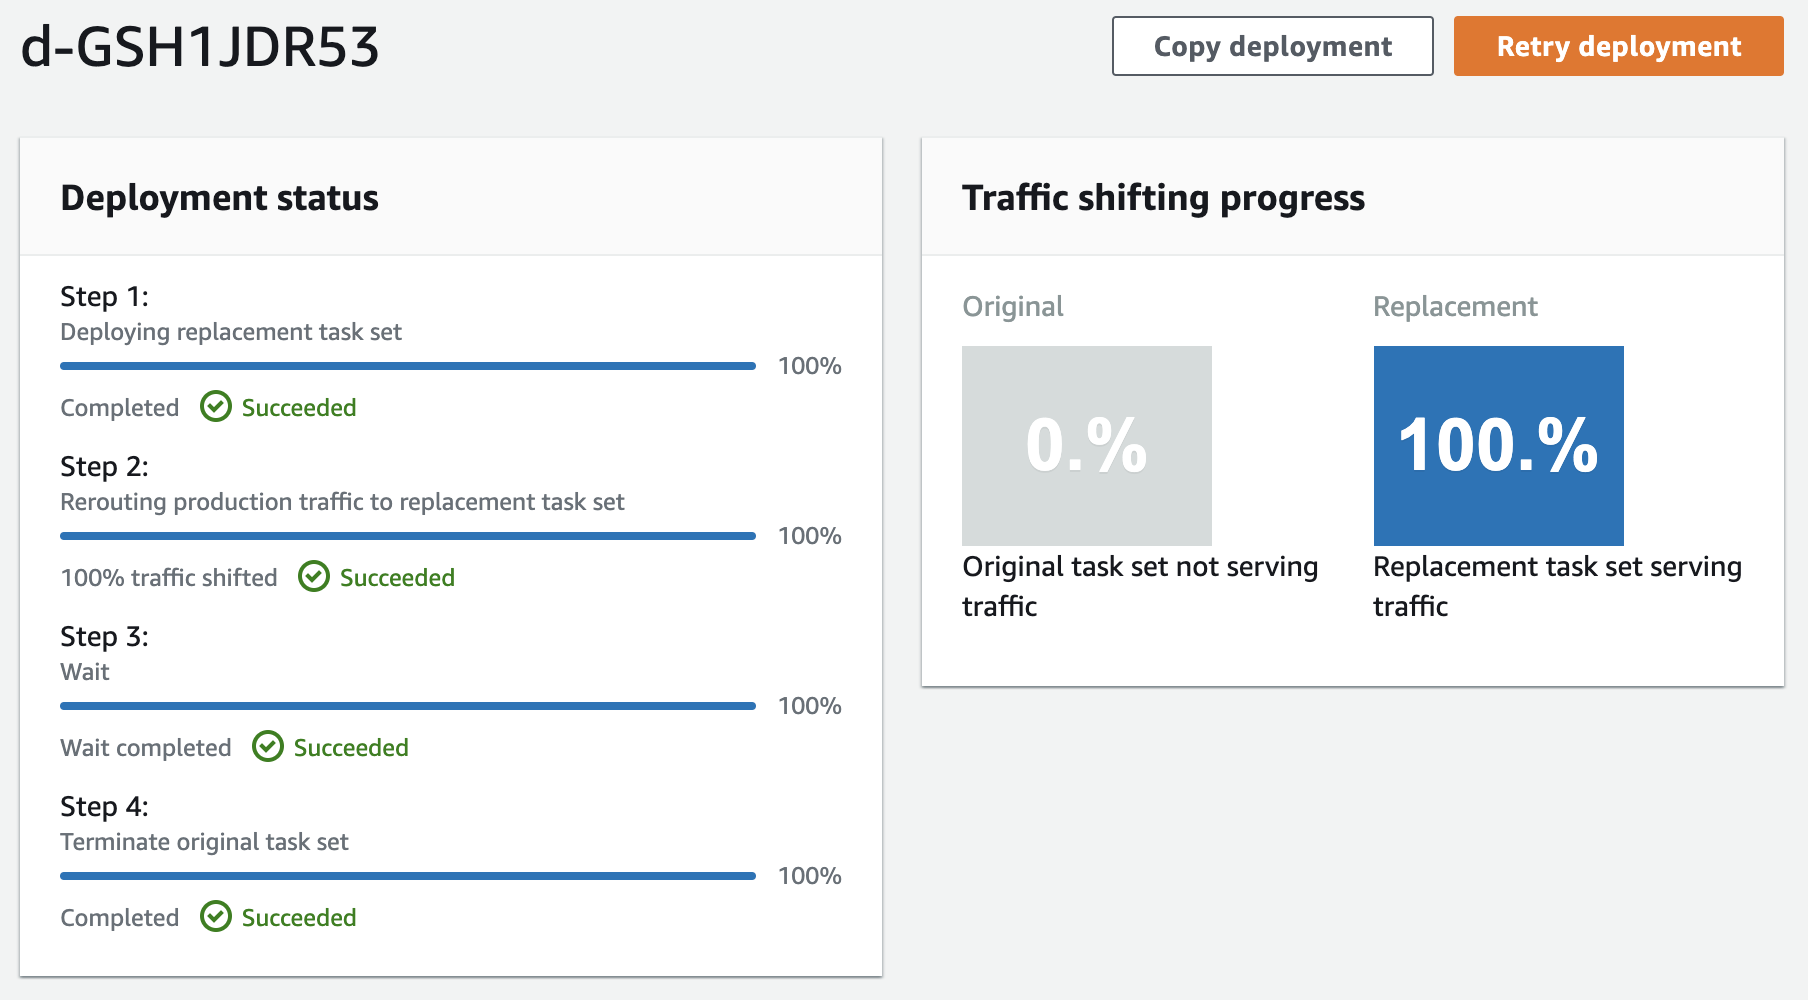
\includegraphics[width=0.90\textwidth]{pics/codedeploy_steps.png}
 \caption{CodeDeploy Dashboard}
 \label{fig:codedeploy_steps}
\end{figure}
\par
The better integration of CodeDeploy with the rest of AWS also brings benefit in the monitoring of the deployed solution. Aside from the existing monitoring with CloudWatch, CodeDeploy also provides us with a dashboard to show the deploy progress and the traffic rerouteing process. Figure \ref{fig:codedeploy_steps} shows the dashboard of CodeDeploy that shows the status of our case project during the deployment.
\par
In comparison, with our non-integrated toolchain, we can not easily do the blue/green deployment. A possible solution is to set up an AWS Lambda function which will be triggered after the deployment. The invoked Lambda function control the load balancer to gradually redirect the traffic from the previous deployment to the new deployment. At the same time, the second lambda function continuously read the health status of the new deployment from the load balancer, and trigger the rollback if the new deployment is unhealthy. Besides all these, a dashboard is needed for developer to monitoring the rerouteing status. On the contrary, in CodeDeploy, all the above tasks are being taken care of.
% \section{Cloud Services}
% \label{assumption}
% In this section, we will introduce several could service from CH3 that could be helpful to the DevOps toolchain. 
% //  Using services in AWS as an example, Introduces how cloud services could improve. describe services in one section
% \subsection{Managed Container Services for Distributed Builds} 

% // Describe how AWS Fargate could Help
% \subsection{Serverless computing}
% // Describe how AWS lambda could Help and why do we choose it
% \subsection{...}
\subsection{Integration of AWS DevOps Tools using CodeStar}
In 4.3.1, we introduce how do we integrate different stages in the continuous delivery pipeline (CD pipeline) with CodePipeline. However, an integrated continuous delivery pipeline is not called integrated toolchain. The DevOps toolchain is centred with the continuous delivery pipelines, but the pipeline is not all of the toolchains. To integrate other AWS tools with the CD pipeline and get the integrated toolchain as a single application, we use CodeStar.  
\par
Figure \ref{fig:codestar} show the user interface of the CodeStar dashboard. We can see, besides the CodePipeline, the CodeStar also integrate tools like monitoring, project management, and version control and then compose our integrated toolchain. In conclusion, the AWS integrated toolchain includes the following tools:
\begin{itemize}
     \item \textbf{CodeStar}: Integrate below tools into a signal toolchain. With project management functionality. The project management could be extended by integrating with third-party tools, i.e. Jira.
          \item \textbf{CodePipeline}: Modelling Continuous Delivery Workflow, integrate tools that used within the CD pipeline.
          \begin{itemize}
               \item \textbf{CodeBuild}: Build code of the software project.
               \item \textbf{CodeDeploy}: Deployment and monitoring.
               \item \textbf{GitHub}: Version control.
          \end{itemize}
          \item \textbf{CloudWatch}: Monitoring deployed solution.
\end{itemize}
\begin{figure}[h]
     \centering
     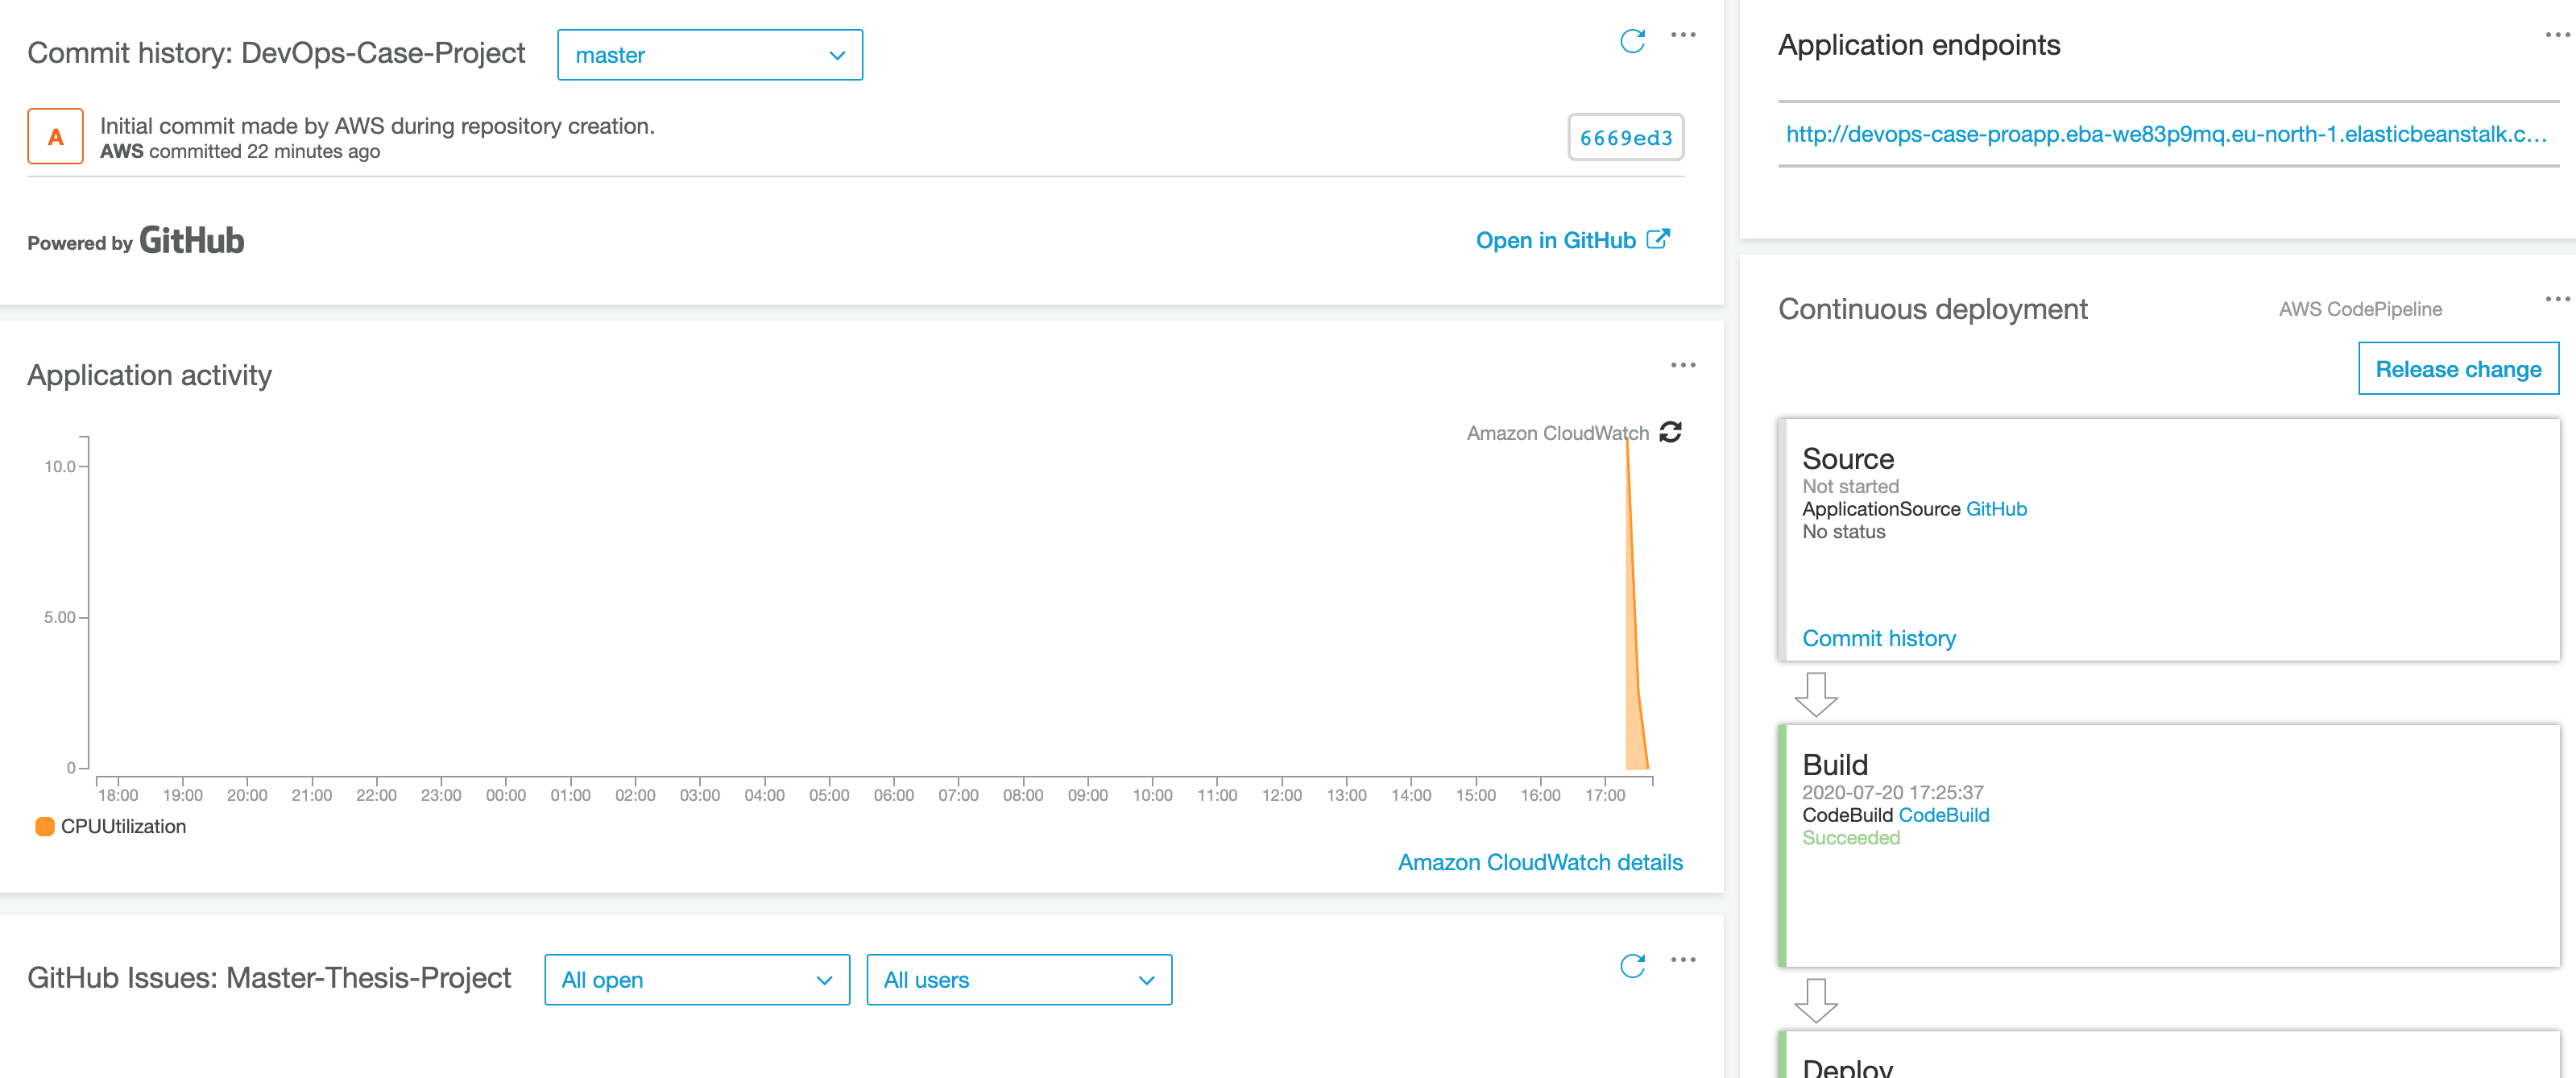
\includegraphics[width=0.99\textwidth]{pics/codestar.png}
     \caption{CodeStar Dashboard}
     \label{fig:codestar}
    \end{figure}

\section{Comparison between Integrated and Non-integrated Toolchain}
In this section, we discuss the difference between these two kinds of toolchains. The scope of comparison will be limited within the scope of functionality and ease of implementation. Furthermore, it is only based on our experiences with the tools used in our implementation.
We summarize the difference between these two toolchains as in Table \ref{tab:toolchain}.
We will do more comparison related to the performance and cost in Chapter 5.
\begin{table}[h]
 \centering
 \begin{tabular}{|c|c|c|}
 \hline
 &
 \begin{tabular}[c]{@{}c@{}}Non-Integrated \\ Toolchain\end{tabular} &
 \begin{tabular}[c]{@{}c@{}}Integrated \\ Toolchain\end{tabular} \\ \hline
    Open-source &
 \begin{tabular}[c]{@{}c@{}}Open-source solution\\ existed\end{tabular} &
 \begin{tabular}[c]{@{}c@{}}No, usually hosted \\ commercial solution\end{tabular} \\ \hline
 \begin{tabular}[c]{@{}c@{}}Delivery \\ method\end{tabular} &
 \begin{tabular}[c]{@{}c@{}}Each part is a stand-alone \\ tool either hosted or\\ on-promised,  depends \\ on the tools selection\end{tabular} &
 \begin{tabular}[c]{@{}c@{}}As a single cloud \\ hosted software\end{tabular} \\ \hline
 \begin{tabular}[c]{@{}c@{}}Implementing \\ time\end{tabular} &
      Long &
      Short \\ \hline
 \begin{tabular}[c]{@{}c@{}}Operational \\ effort\end{tabular} &
      High &
      Low \\ \hline
 \begin{tabular}[c]{@{}c@{}}Visibility \\ on status\end{tabular} &
 \begin{tabular}[c]{@{}c@{}}Depends on tools, a \\ well-integrated toolchain \\ could gives good overview\\ on the whole toolchain.\end{tabular} &
 \begin{tabular}[c]{@{}c@{}}Easy to see the\\ status as a whole\\ without additional \\ implementation\\ effort, low visibility\\ on under-laying \\ server since it's \\ hosted solution\end{tabular} \\ \hline
 \begin{tabular}[c]{@{}c@{}}Extendibility\\ and tool \\ selection\\ freedom\end{tabular} &
 \begin{tabular}[c]{@{}c@{}}Free to select tools\\ for each part of the\\ toolchain.\end{tabular} &
 \begin{tabular}[c]{@{}c@{}}Limited integration\\ with third-party \\ tools\end{tabular} \\ \hline
 \end{tabular}
 \caption{Comparison of continuous delivery tools}
 \label{tab:toolchain}
 \end{table}
\subsection{Implementation and Cloud Deployment}
The cloud based integrated toolchain is delivered as hosted solution in a serverless model. However we noticed that the non-integrated toolchain could be also completely serverless if we using hosted tools for all the components. 
\par
For example in our solution, we only have continuous integration pipeline which is on-promised and need to be deployed to the VM manually. If we replace Jenkins with some other hosted tools, for example, Travis CI\footnote{https://travis-ci.org/} we can actually build a fully hosted but non-integrated DevOps toolchain. But, for following reasons, it is not a satisfactory solution thus a non-integrated toolchain usually has some on-promised modules that needs operational effort and cloud knowledge.
\begin{itemize}
 \item The hosted tools, especially tools for continuous integration pipeline, are all closed-source commercial solution. This means there is no community support like in Jenkins, and it can usually integrates with the certain tools that supported by vendor. Besides, commercial user always need to pay for these hosted tools.
 \item Hosted tools runs in the vendor's server, and it requests user log in to use this tool which brings extra integration difficulty. This means for two hosted toolchain to integrated with each other, it not only need to do the integration in the data transfer, but also need to connect their account system, for example, with OAuth. This extra inconvenience makes most hosted DevOps tools only do the integration support with other most most popular tools which largely limited the extendibility.
\end{itemize}
Therefore, a non-integrated toolchain usually has some on-promised module in real-life use. In our deployment process, we find it requires lot of work to put an on-promised tool to cloud, especially if the developer is not familiar with the cloud platform that deploy this tools. For only deploying Jenkins we need to do following steps:
\begin{enumerate} 
 \item Create a cloud virtual machine (EC2 instances) for hosting the Jenkins master.
 \item Setup IAM role for Jenkins master VM, make sure it has access to other AWS recourse that needed during build.
 \item Setup security group and networking for the VM, makes sure it can be accessed form the internet but only accessible within company's IP range, and only port needed are opened to the public.
 \item Install Jenkins in the VM. Research what plugin is needed and install necessary plugins.
 \item An tedious set-up process for setup Jenkins cluster that supports the distributed build. This includes setup ECS cluster for build agent. Although Terraform makes the provision of cloud resources easier, still, prior knowledge for AWS is needed. The experiences in AWS is also needs to correctly configure ECS cluster that maximizing the performance of build agents.
 \item Develop Docker image for the container that runs Jenkins agents.
 \item Setup integration with other tools in toolchains by finding correct plugins and configure these plugins. 
\end{enumerate}
Only after these steps, we can start using Jenkins as part of our toolchain.
In comparison, the core feature of the integrated toolchain in AWS is an out-of-the-box feature which means there is no previous cloud knowledge needed, and there is no deployment and environment configuration required before we use it. We are free from all the steps we mentioned above.
\subsection{Extendibility and Flexibility}
The integrated toolchain is a hosted platform that runs by a vendor. Similar to we mentioned in 4.4.1, We find all the currently integrated toolchain are all commercial and closed-source which has no community support. So the integration of their third-party tools usually only limited to popular tools. For example, AWS DevOps tools only support 21 tools within it is "DevOps Partner Solutions" \footnote{https://aws.amazon.com/devops/partner-solutions/}. If the user wants to use anything except these tools, it is not possible.
\par
Nevertheless, different with the single hosted tools we mentioned in 4.1.1, a hosted integrated DevOps toolchain mostly has everything needed for DevOps lifecycle, so it is not mandatory for it to able to integrates with third-party tools. Still, the limitation in third party tool support might make the software team facing trouble when they want to use certain tools which are not very supported.
\par
A non-integrated toolchain allows the software team to pick any tools for each component, as long as those tools can be integrated. The tools in the toolchains could also be open-source, which allow so the software team modify the tools according to their need. For example, develop a plugin for Jenkins that allows the integration of internal company tool with Jenkins.
\par
In conclusion, in terms of extendibility and flexibility, non-integrated toolchains are better than integrated toolchain.
\subsection{Integration Between Tools}
As we mentioned in 4.4.1, sometimes it is hard for tools within a non-integrated toolchain to integrate, especially between the hosted tools. 
During our implementation, we also realized that, first, it requires some configuration work for tools to be able to work together. Secondly, sometime the Integrated could be buggy, for example, in our toolchain, the Jenkins sometimes does not react to the build triggering signal from GitHub. This means the software teams need further maintaining of the toolchain.
In integrated toolchain, the toolchains are delivered as a single cloud-based software, each part of naturally coped with each other, which makes integration much more straightforward.
The better integrating between each component also makes it easier to monitor the toolchain as a whole.
\subsection{Visibility}
\label{visibility}
In 4.4.3, we mentioned that the integrated toolchain is easier to be monitored as a whole, however, when comes to every single component, in our implementation, we find out that integrated toolchain is lack of visibility. We met two difficulties when test two toolchain. The first one is that Jenkins master was having difficulty in the provision and connect to the agents. Since Jenkins is a web service deployed in our EC2 virtual machine, We solve the problem by reading the Error message within the Jenkins log file. The second problem we met was within AWS CodeDeploy. The CodeDeploy failed to deploy the case project to the ECS cluster. We could not find the reason at that time since we cannot find the log of CodeDeploy anywhere since it is not shown in the web interface, and we have no access to the underlying cloud infrastructure either. The lack of visibility is a problem with all hosted serverless services since the users do not have the visibility to the infrastructure behind the service.

\section{Challenges in Implementation and Design of DevOps toolchains}
In this section, we discuss the challenge that we met during the implementation. 
\subsection{Challenge I: The Enormous and Unregulated Jenkins Plugins System}
Jenkins has more than 1600 plugins which brings the software an amazing extendibility, which is one of the main advantages of Jenkins. However, there are two problems with Jenkins' plugins; First, there are usually more than one plugins that have the same functionality, for example, there are at least five different plugins related to running Docker container as Jenkins agent. Second, most of the plugin is developed by the open-source community, so the quality of these plugins is not ensured. During our implementation, we find out there are two plugins that support run Jenkins agent in ECS cluster. However, we find only one work after we tried both plugins. Besides, the documentation of Jenkins plugins sometimes is abysmal. For example, the documentation of the plugin that we use for Jenkins agent is too brief to tell us how to use the plugin, and it is not even mentioned the security setting needed in Jenkins master node that allows agents to connect the master node. 
\par
As a result of the above three factors, we spent a very long time in selecting and configuring tools. Moreover, trying to solve the problem which nether mentioned in the documentation and on the internet. 
\subsection{Challenge II: Fargate Does not Supports Container runs in Privileged Mode}
As said per title, this is some limitation in AWS Fargate for preventing container get permission to access the critical resource on the host(underlying server hosting Fargate instances in this case). As a result, we cannot use Docker within a Docker container that runs on Fargate. This makes it impossible for us to distribute the "Build docker image" and "Push to ECR" stages to agents. Instead, we have to run them on the master. Luckily, these two stages take a short time (<5s in total), so this limitation will not slow down the pipeline too much when multiple builds run in parallel.
\par
A possible solution solving this problem is to runs these two stages in AWS CodeBuild, AWS CodeBuild has support to Jenkins, which allow us to run certain Jenkins stages in CodeBuild. Moreover, CodeBuild supports fully parallel execution as in Fargate.
\subsection{Challenge III: Slow Starting Time for Agents in AWS Fargate}
On average it takes around 60s from sending a Jenkins job to agent, to running the job in an agent. To our case project that takes 90 seconds to go through the whole pipeline, this is a relatively long time. During this 60s, Jenkins master node sends task definition \footnote{Define specification of a container runs in ECS.} to ECS, provision a Fargate instance within ECS, then pull the image we developed for Jenkins agent, star the agent container within Fargate and then connect to the Jenkins master. This challenge is due to the nature of the serverless computing that we discussed in Chapter 2, and we believe there is not an economical way to solve the challenge with the current setup.
\subsection{Challenge IV: No Enough Visibility in AWS DevOps tools}
As we mentioned in \ref{visibility}, the lack of visibility to the underlying process, especially in CodeDeploy, caused some obstacle for us to debugging our pipeline. There was a problem when we try to deploy the case project to the ECS with blue/green deployment, and the CodeDeploy sucked in the creating replacement service. We know there was something wrong within either the configuration of ECS, load balancer, health-check or security/network setting. Nevertheless, there is no log output of the underlying deployment process in CodeDeploy. In the end, we have to check everything that might be caused problem one by one and found it was the problem with failed health-check, which was very time-consuming.